\documentclass[11pt]{article}
\PassOptionsToPackage{breaklinks,colorlinks=true,linkcolor=blue}{hyperref}
\newif\ifLoMEDBibStyleSet
\let\LoMEDOriginalBibStyle\bibliographystyle
\renewcommand{\bibliographystyle}[1]{\ifLoMEDBibStyleSet\else\global\LoMEDBibStyleSettrue\LoMEDOriginalBibStyle{#1}\fi}
\usepackage[review]{acl}
\usepackage[T1]{fontenc}
\usepackage[utf8]{inputenc}
\usepackage{times}
\usepackage{latexsym}
\usepackage{microtype}
\IfFileExists{inconsolata.sty}{\usepackage{inconsolata}}{}
\usepackage{array,booktabs,colortbl}
\usepackage{amsmath}
\usepackage{amssymb}
\usepackage{xcolor}
\usepackage[edges]{forest}
\usepackage{mathtools}
\usepackage{array}
\newcolumntype{q}[1]{>{\raggedright\arraybackslash}p{#1}}
\usepackage{amsthm}
\usepackage{graphicx}
\usepackage{subcaption}
\usepackage{tabularx}
\usepackage{booktabs}
\usepackage{multirow}
\usepackage{makecell}
\usepackage{colortbl}
\usepackage{xcolor}
\usepackage{enumitem}
\usepackage{placeins}
\usepackage{flafter}
\usepackage{tikz}
\usetikzlibrary{matrix,positioning,arrows.meta,fit}
\usepackage[edges]{forest}
\usepackage{pgfplots}
\pgfplotsset{compat=1.18}
\usepgfplotslibrary{groupplots}
\usepackage{pgfplotstable}
\IfFileExists{algorithm.sty}{\usepackage{algorithm}}{}
\IfFileExists{algpseudocode.sty}{\usepackage{algpseudocode}}{}
\usepackage{listings}
\lstset{ basicstyle=\ttfamily\scriptsize, breaklines=true, columns=fullflexible, frame=single, showstringspaces=false
}
\usepackage{pifont}
\usepackage[capitalize,noabbrev]{cleveref}
\usepackage[textsize=tiny]{todonotes}
\usepackage[most]{tcolorbox}
\usepackage{caption}
\captionsetup{font=small,skip=2pt}
\definecolor{tableheader}{RGB}{230,240,255}
\definecolor{tablerow}{RGB}{245,248,255}
\definecolor{linkblue}{RGB}{0,0,255}
\definecolor{gain}{RGB}{0,120,0}
\definecolor{loss}{RGB}{180,0,0}
\definecolor{headergray}{RGB}{235,235,235}
\definecolor{sectiongray}{RGB}{245,245,245}
\definecolor{stagegray}{RGB}{240,240,240}
\definecolor{datablue}{RGB}{20,90,160}
\definecolor{trainpurple}{RGB}{120,40,140}
\definecolor{resultgreen}{RGB}{0,120,60}
\definecolor{hidden-draw}{RGB}{20,68,106}
\definecolor{leafgray}{RGB}{248,248,248}
\newcommand{\cmark}{\ding{51}}
\newcommand{\xmark}{\ding{55}}
\newcommand{\gup}[1]{{\color{gain}\scriptsize$\uparrow$#1}}
\newcommand{\rdown}[1]{{\color{loss}\scriptsize$\downarrow$#1}}
\newcommand{\xref}[2]{
\hyperref[#1]{\underline{\textcolor{blue}{#2~\ref*{#1}}}}}
\newcommand{\xrefn}[1]{
\hyperref[#1]{\underline{\textcolor{blue}{\ref*{#1}}}}}
\theoremstyle{plain}
\newtheorem{theorem}{Theorem}[section]
\newtheorem{proposition}[theorem]{Proposition}
\newtheorem{lemma}[theorem]{Lemma}
\newtheorem{corollary}[theorem]{Corollary}
\theoremstyle{definition}
\newtheorem{definition}[theorem]{Definition}
\newtheorem{assumption}[theorem]{Assumption}
\theoremstyle{remark}
\newtheorem{remark}[theorem]{Remark}
\title{A Cross-Domain Survey of Longitudinal Modeling Approaches, Evaluation Practices, and Datasets}
\author{Anonymous submission}
\begin{document}
\maketitle
\begin{abstract}
Longitudinal NLP increasingly applies long-context models and large language models (LLMs) to user timelines, yet seeing more history is not the same as modeling how it temporally changes. We survey 172 studies from IEEE Xplore and the ACL Anthology \footnote{\small ACL, AACL, COLING, EACL, EMNLP, LREC, NAACL, TACL} across clinical, behavioural, and language data. We identify five dimensions important to all longitudinal studies: the length and order in a timeline, the time between observations, tackling missing observations, changes in a subject's state, and alignment across data types. We report trends along each dimension, distinguish families of methods and how they address each dimension, and examine how studies are evaluated. Sequential modeling appears in 86.6\% of studies, but 59.3\% state no strategy for missing observations, only 11.0\% test on later time points, and 4.1\% test on prospective data. We map each study's claims to the corresponding necessary validation checks (e.g., claims about progression require testing on later time points), finding that only 89 of 390 required checks (22.8\%) are performed, and 112 of 171 studies (65.5\%) perform none. We separate challenges shared by all longitudinal data from those specific to text and multimodal data, and recommend models that represent elapsed time and change, together with evaluation matched to the generalization a study claims. \textsc{Webpage}\footnote{\url{https://anonymous.4open.science/w/Multimodal-Longitudinal-Dataset-Survey/}}
\end{abstract}

\section{Introduction}
\label{sec:introduction}

% --- What longitudinal modeling is ---
Longitudinal datasets link observations of the same individuals or entities over time, enabling the study of progression, recurrence, and change~\cite{diggle2024longitudinal}. While longitudinal NLP and multi-modal datasets remain underrepresented, there is a recent increase, particularly involving user timelines, where the goal is to track the user progression~\cite{tsakalidis-etal-2022-overview}. Predicting clinical outcomes over time from patients' history~\cite{rajkomar2018scalable}, provided in a structured form, is a standard longitudinal task. %Clinical prediction from patient history~\cite{rajkomar2018scalable} shares this structure in a much larger literature. 
Whether based on structured or unstructured data, longitudinal tasks share common objectives: to infer what changes, for whom, and over what interval. The \emph{observation regime}, i.e., how and when observations of a subject are collected and how regular and complete they are, constrains what a model can learn. For example, missed clinical visits leave incomplete measurements that require decisions about missing values~\cite{8904478}, while scheduled brain scans can provide spatial evidence of change~\cite{10483639}. Social-media timelines reveal selectively expressed states~\cite{coppersmith-etal-2016-exploratory}, and timeline summarization must select and order evidence across a history~\cite{wu-etal-2025-unfolding,song-etal-2025-temporal}. 
% The observation regime thus shapes both modeling choices and what a successful prediction shows. 

Architectures have steadily extended how much history a model sees: RNNs update a state sequentially, transformers can attend more successfully to distant positions~\cite{vaswani2023attentionneed}, Longformer uses sparse attention for long documents~\cite{beltagy2020longformer}, and large language models (LLMs) process long histories within extended context windows~\cite{brown2020language,bommasani2022opportunitiesrisksfoundationmodels}. Longitudinal NLP reflects this, with shared tasks on evolving mental-health trajectories~\cite{tseriotou-etal-2025-overview,ali-etal-2026-overview, soni-etal-2026-semeval}, prompting with long histories \citep{kruse-etal-2025-large} and instruction-tuning LLMs for longitudinal in-context prediction~\cite{ali2026liftenableincontextlearning, cui2025timer}. Yet longer context windows do not inherently enable longitudinal reasoning; a model may treat a timeline as a single document rather than capturing progression over time. Although models can process longer histories, whether they do so longitudinally remains undemonstrated. Studies differ in objectives, validation, and length of historical context, so their claims are hard to compare. Temporal shifts affect language-model evaluation~\cite{lazaridou2021mindgapassessingtemporal}, irregular and missing observations need explicit assumptions~\cite{perveen2020handling,bazo2020handling}. Moreover, work on user-generated content must account for temporal dynamics~\cite{tabak2020temporalmentalhealthdynamics}, label validity over time~\cite{harrigian-dredze-2022-now}, evaluation on user-aware temporal splits~\cite{ganesan2026word} and increasingly, multiple evolving streams~\cite{hills-etal-2026-multistream}. Random splits of pooled timelines can yield high accuracy with no evidence of future-time or cross-dataset generalization~\cite{tsakalidis2018can}. We therefore examine whether reported evaluation matches a study's claims to generalisability.

% --- Positioning and scope ---
\noindent\emph{\textbf{Positioning and scope:}} Prior reviews cover single domains: biomedical data~\cite{cascarano2023machine}, electronic health records (EHRs)~\cite{xie2022deep,carrasco2023prediction}, multimodal clinical data~\cite{pan2026systematic}, radiology~\cite{zhou2025review}, time series~\cite{jin2026large}, or longitudinal NLP evaluation~\cite{ganesan2026word}. % broader 
Surveys on multimodal learning~\cite{xu2024comprehensive} focus on how modalities are combined but not on their alignment when observed at different times. Surveys on temporal information retrieval and question answering~\cite{piryani2025itshightimesurvey} address time mentions in documents and queries rather than longitudinal observations. None jointly assess datasets, models, and evaluation across the dimensions shared by all longitudinal tasks. While focusing on NLP, we draw from the clinical and multimodal literature (clinical tabular data accounts for 36.0\% of studies) to highlight what longitudinal language modeling should adopt and avoid (Fig. \ref{fig:overview}), as we uncover systematic validation gaps: ACL Anthology studies use temporal splits more often than IEEE Xplore (26.5\% vs.\ 7.2\%). %, but none report external validation. 
Our contributions are:
\begin{itemize}[leftmargin=*,nosep,labelsep=1em]
\item \emph{\textbf{Dimensions/aspects of longitudinal modeling:}} We identify five aspects related to temporality, that every longitudinal study must handle: the length and order of historical content, the time between observations, missing observations, changes of outputs over time (e.g. user states), and alignment across data types (\S\ref{sec:survey_design}).
\item \emph{\textbf{Trends along each dimension:}} Coding 172 clinical, behavioral, and language studies with a shared rubric, we report how datasets and tasks vary along each dimension (\S\ref{sec:data_landscape}).
\item \emph{\textbf{Method families:}} For each dimension, we describe the main families of methods, how they handle corresponding challenges, and where they fall short, providing examples (\S\ref{sec:modeling}).
\item \emph{\textbf{Evaluation and its limits:}} We describe how longitudinal models are being evaluated and show that evaluation rarely tests the kind of generalisability a study claims (\S\ref{sec:evaluation}).
\item \emph{\textbf{Challenges and recommendations:}} We separate challenges shared by all longitudinal data from those specific to text and multimodal data, and propose directions for future work (\S\ref{sec:open_challenges}).
\end{itemize}
\begin{table*}[!t]
\centering
\footnotesize
\setlength{\tabcolsep}{3pt}
\renewcommand{\arraystretch}{1.05}
\rowcolors{2}{gray!6}{white}
\begin{tabularx}{\textwidth}{@{}>{\raggedright\arraybackslash\bfseries}p{2.15cm}>{\raggedright\arraybackslash}p{2.8cm}>{\raggedright\arraybackslash}p{1.8cm}>{\raggedright\arraybackslash}p{3.45cm}>{\raggedright\arraybackslash}X@{}}
\toprule
\rowcolor{gray!18}
\textbf{Task} & \textbf{Modalities; temporal signal} & \textbf{Scope} & \textbf{Typical models} & \textbf{Example tasks; evaluation} \\
\midrule
Trajectory classification & Text, image, physiology; evolving states & Long-range & Transformers, LLMs, CNNs~\cite{vaswani2023attentionneed,brown2020language} & Mood/disease progression; subject splits, calibration, external validation~\cite{rajkomar2018scalable,piryani2025itshightimesurvey} \\
Transition detection & Text, audio, video; state change & Local + context & RNNs, long-context transformers~\cite{10796324,beltagy2020longformer} & State-change detection; transition precision/recall, chronology~\cite{tsakalidis-etal-2022-identifying,lazaridou2021mindgapassessingtemporal} \\
Forecasting & Physiology, text; sparse or irregular & Forward & GRUs, neural ODEs, transformers~\cite{9338417,9374359} & Risk forecasting; horizon-aware metrics, leakage control~\cite{rajkomar2018scalable} \\
Temporal summarization & Text, multimodal records & Sequence-wide & Long-context LLMs~\cite{li2024long,qiu-etal-2024-large} & Timeline summaries; faithfulness, chronology~\cite{wu-etal-2025-unfolding,matero-etal-2024-using} \\
Representation learning & All modalities; global structure & Global & VAEs, contrastive, sequential~\cite{9761588,10385940} & Temporal embeddings, biomarkers; transfer robustness \\
Multimodal progression & Cross-modal, asynchronous & Cross-modal, temporal & Report generation, fusion~\cite{serra-etal-2023-controllable,10313489} & Progression, risk; modality dropout, alignment~\cite{10385940,10890535} \\
\bottomrule
\end{tabularx}
\caption{\textit{Longitudinal task families} used to group the coded studies (a study may belong to several): the temporal signal each relies on, how much history it uses (scope), typical models, and the evaluation its claims require. The evaluation column states recommended evidence, not observed prevalence; citations are illustrative.}\label{tab:unified_longitudinal_taxonomy}
\end{table*}

\noindent Table~\ref{tab:unified_longitudinal_taxonomy} outlines the scope; \S\ref{sec:survey_design} covers study selection \& coding, \S\ref{sec:data_landscape} data trends, \S\ref{sec:modeling} method families, \S\ref{sec:evaluation} evaluation, and \S\ref{sec:open_challenges} challenges.
\section{Survey Design and Scope}
\label{sec:survey_design}
%\noindent\textbf{Research questions:} 
This review addresses four \textbf{research questions:}\\ 
\textbf{RQ1:} Which observation regimes do longitudinal datasets follow across domains, and what temporal evidence does each make available to a model? Here \emph{observation regime} denotes how a dataset's observations accumulate (e.g. scheduled visits, irregular events, self-selected posts) and \emph{temporal evidence} denotes what those observations reveal about time (e.g. ordering, elapsed time).\\
\textbf{RQ2:} How do modeling approaches represent time: do they encode ordering, elapsed time, and state change, or only process longer histories?\\
\textbf{RQ3:} Does the reported evaluation support a study's claims of generalisability, both in terms of protocol (e.g. via subject-disjoint designs such as leave-one-user-out, temporal splits, external and prospective validation) and metrics (e.g. static versus transition- or horizon-sensitive)?\\
\textbf{RQ4:} What methodological gaps limit longitudinal modeling, and what should language-based longitudinal modeling adopt or avoid from the clinical and multimodal literature?\\
\noindent\textbf{Constructing a comparison framework and why it is needed:} Answering the RQs requires comparing studies that share no dataset, task, or architecture (e.g., an MRI classifier vs.\ a change detector on social media); grouping them by domain or model family misses important elements such as evaluation. We therefore describe each study along five interconnected aspects, \emph{(1) observation regime $\rightarrow$ (2) temporal evidence $\rightarrow$ (3) temporal objective $\rightarrow$ (4) model inductive bias $\rightarrow$ (5) evaluation requirement} (Fig \ref{fig:taxonomy_logic}), ordered by dependency: what observations reveal about time limits the task, and the task determines the model and evaluation needed. Aspects 1--4 are  recorded for every paper (Table~\ref{tab:taxonomy_operationalization}); for example, a study's observation regime follows from its dataset, modality, and whether it reports irregular intervals or missing visits, so an ICU study on MIMIC with irregular intervals is classed as event-driven. Aspect 5 states what evaluation a study \emph{should} report given its claims, using fixed rules: a study claiming to predict disease progression requires testing on later time points (a temporal split), and one claiming to generalise to new patients requires a subject-disjoint split. We then compare these requirements with the evaluation each study \emph{actually} reports. Aspects 1--2 address RQ1 (\S\ref{sec:data_landscape}), 3--4 address RQ2 (\S\ref{sec:modeling}), and 5 addresses RQ3 (\S\ref{sec:evaluation}); mismatches across aspects inform RQ4 (\S\ref{sec:open_challenges}).\\
\noindent\textbf{Sources and screening:} We collected English-language full papers from two complementary sources: the ACL Anthology {\small (ACL, AACL, COLING, EACL, EMNLP, LREC, NAACL, and TACL)}, which archives the main NLP venues, and IEEE Xplore, which indexes the engineering and computational-health venues where longitudinal modeling is most established. The window spans January 2019, beginning after the widespread adoption of pretrained transformers, to October 2026. Of 875 records, 591 passed automated filtering, 555 passed manual screening, and 174 were retained after full-text review; removing two duplicate records leaves 172 unique studies (Appendix~\ref{sec:appendix_sources}--\ref{sec:appendix_screening}). The corpus is imbalanced (IEEE Xplore, 80.2\%; ACL Anthology, 19.8\%), so aggregates describe the paired sample; stratified rates are in Table~\ref{tab:crossdim_validation} and Appendix~\ref{sec:appendix_source_analysis}.\\
\noindent\textbf{Coding.} One reviewer coded all 172 papers from the full text (data, models, temporal challenges, evaluation, reproducibility), recording the supporting passage for each label; a second reviewer piloted the codebook on 12 studies (\S\ref{sec:limitations}; Appendices~\ref{sec:appendix_extraction}--\ref{sec:appendix_operational_definitions}). \emph{Corpus-wide} rates use 172 studies (e.g., 11.0\% use temporal splits); \emph{conditional} rates use the relevant subset and state its denominator (e.g., 10.1\% of 149 sequential-modeling studies).


\providecolor{hidden-draw}{RGB}{20,68,106}
\providecolor{leafgray}{RGB}{248,248,248}
\providecolor{evalgreen}{RGB}{0,110,60}
\providecolor{datablue}{RGB}{20,90,160}
\providecolor{trainpurple}{RGB}{120,40,140}

\newcommand{\LMcue}[1]{%
  \textcolor{hidden-draw}{\textbf{#1}}\,\textbar\,}
\newcommand{\LMdata}[1]{%
  \textcolor{datablue}{\textbf{D}\,\textit{(#1)}:}~}
\newcommand{\LMmethod}{%
  \enskip\textcolor{trainpurple}{\textbf{M:}}~}
\newcommand{\LMeval}{%
  \enskip\textcolor{evalgreen}{\textbf{E:}}~}
\begin{figure*}[t]
\centering
\begin{forest}
forked edges,
for tree={
  grow=east,
  reversed=true,
  anchor=west,
  parent anchor=east,
  child anchor=west,
  font=\fontsize{6.5}{7.6}\selectfont,
  rectangle,
  draw=hidden-draw,
  rounded corners,
  node options={align=left},
  edge={darkgray, line width=0.4pt},
  s sep=1.5pt,
  l sep=5pt,
  inner xsep=2pt,
  inner ysep=1.5pt,
  outer sep=0pt,
  line width=0.4pt,
},
where level=0{
  text width=1.35cm,
  fill=blue!6,
  font=\fontsize{6.5}{7.6}\selectfont\bfseries
}{
  text width=\dimexpr\textwidth-1.35cm-14pt\relax,
  fill=leafgray,
  draw=blue!35
},
[Language \&\\behavioural\\histories
  [{\LMcue{State change}
    \LMdata{activity-driven} TalkLife, CLPsych.
    \LMmethod BiLSTM--BERT detects switches and escalations.
    \LMeval Change windows; exclude future posts for early warning.}]

  [{\LMcue{Language trajectories}
    \LMdata{activity-driven} TalkLife, Reddit.
    \LMmethod Seq-Sig-Net models language histories.
    \LMeval Cross-dataset tests.}]

  [{\LMcue{Label validity \& shift}
    \LMdata{activity-driven} Reddit mental-health histories.
    \LMmethod Temporal dynamics modelling.
    \LMeval Label validity; future-period tests.}]

  [{\LMcue{Within-person change}
    \LMdata{scheduled; within-session} LoSST-AD, EMINDS, AnnoMI.
    \LMmethod Lexical and interaction analysis.
    \LMeval Within-subject analysis.}]

  [{\LMcue{Timeline summarisation}
    \LMdata{document timeline} Open-TLS, annotated user timelines.
    \LMmethod Timeline summarisation.
    \LMeval Faithfulness; chronology consistency.}]

  [{\LMcue{LLM temporal reasoning}
    \LMdata{mixed} TimeBench, long-context benchmarks.
    \LMmethod Prompting, retrieval, memory.
    \LMeval Shuffled-history and timestamp-removal controls.}]
]
\end{forest}

\caption{%
\textbf{Connecting temporal evidence, methods, and evaluation:} Language and behavioural histories linking
\textcolor{datablue}{\textbf{D}}ata,
\textcolor{trainpurple}{\textbf{M}}ethods, and
\textcolor{evalgreen}{\textbf{E}}valuation
(framework aspects 1, 4, and 5; \S\ref{sec:survey_design}).
Full map and references in Appendix Figure~\ref{fig:literature_map_full}.}
\label{fig:literature_map}
\end{figure*}
% \begin{figure*}[t]
% \centering
% \providecolor{hidden-draw}{RGB}{20,68,106}\providecolor{leafgray}{RGB}{248,248,248}\providecolor{evalgreen}{RGB}{0,110,60}\providecolor{datablue}{RGB}{20,90,160}\providecolor{trainpurple}{RGB}{120,40,140}
% \newcommand{\mech}[1]{\textcolor{hidden-draw}{\textbf{#1}}\,\textbar\,}
% \newcommand{\D}[1]{\textcolor{datablue}{\textbf{D}\,\textit{(#1)}:}~}
% \newcommand{\M}{\enskip\textcolor{trainpurple}{\textbf{M:}}~}
% \newcommand{\E}{\enskip\textcolor{evalgreen}{\textbf{E:}}~}
% \begin{forest}
% forked edges,
% for tree={
%   grow=east, reversed=true, anchor=base west, parent anchor=east, child anchor=west,
%   base=left, font=\fontsize{6.5}{7.6}\selectfont, rectangle, draw=hidden-draw, rounded corners,
%   edge+={darkgray, line width=0.45pt}, s sep=0.6pt, l sep=3pt,
%   inner xsep=1.5pt, inner ysep=0.6pt, line width=0.4pt,
% },
% where level=0{rotate=90, child anchor=north, parent anchor=south, anchor=center, font=\scriptsize\bfseries}{},
% where level=1{text width=1.35cm, node options={align=left}, fill=blue!6, font=\fontsize{6.5}{7.5}\selectfont\bfseries}{},
% where level=2{text width=13cm, node options={align=left}, fill=leafgray, draw=blue!35}{},
% [Longitudinal data and methods
%   [Clinical\\cohorts
%     [{\mech{Cohort resources}\D{scheduled} ADNI (6--12-mo visits; 24/172 studies), OASIS (3--5 visits; 7), AIBL (18-mo), ABCD ($\sim$11.8K; 4), UK Biobank (500K+), FHS, NACC \M cohort modeling \citep{9098513,10635331,10635830}; missing visits, attrition, heterogeneity \citep{9342532,10415852,9374343,8759198,10635519,9983643,10069449} \E subject-disjoint splits, calibration, external cohorts}]
%     [{\mech{Feature recency}\D{scheduled waves} ELSA: biennial, 4 waves, 7,096 participants, 140 features \M \textbf{Lexicographic RF} prefers recent features at near-tied gain; higher sensitivity, no geometric-mean gain \citep{9308198}; SVM/LASSO \citep{9377173,8857827}; feature learning \citep{9313310,9629798,10822368} \E metric-specific reporting}]
%     [{\mech{Incomplete follow-up}\D{scheduled, incomplete} CLIMB: repeated multiple-sclerosis assessments \M \textbf{GRU-DF} fills missing lagged targets \citep{9374359}; recurrent models \citep{10796324,8834556}; continuous-time, missingness-aware updates \citep{9871150,10340079} \E imputation and forecasting scored separately}]
%     [{\mech{Imaging trajectories}\D{scheduled} ADNI, OASIS, AIBL MRI; PPMI annual (4) \M \textbf{LongFormer}: 3D CNN + transformer over scans and deformation flows \citep{10483639}; progression \citep{8857827,9669504,10489807,10959402,10340372} \E forecasting protocol; ADNI$\rightarrow$AIBL transfer}]
%     [{\mech{Latent progression}\D{scheduled} high-dimensional multimodal cohorts \M VAEs, GANs, diffusion, neural ODEs \citep{9338417,9761641,9761588,10635663,9630495,9669504}; digital twins \citep{9098571,9008303,9669428}; compute cost \citep{8885357,8730775} \E interpolation vs.\ forecasting}]
%   ]
%   [Clinical\\records (EHR)
%     [{\mech{Irregular events}\D{event-driven} MIMIC-III/IV/CXR (15/172; 60K+/70K+), eICU (200K+), N3C, OptumLabs \M RNNs, neural ODEs, transformers for outcomes \citep{rajkomar2018scalable,8904478,9006400,9679113,beaulieu2018mapping,teoh2026predicting,9926878,9623284,8904622,9874605,9313227} \E chronological, horizon-aware splits}]
%     [{\mech{Long notes}\D{event-driven} MIMIC-III notes aggregated within visits \M \textbf{ClinicalMamba}: state-space LM for long histories, not elapsed time \citep{yang-etal-2024-clinicalmamba} \E timestamp and order ablations}]
%     [{\mech{Multi-site \& privacy}\D{event-driven} multi-institution records; multi-site validation 1.2\% \M federated training \citep{9983621}; DP/synthetic data \citep{9474660,10821737}; access limits \citep{10494110,10507968,8730775} \E cross-site, cross-time tests}]
%   ]
%   [Language \&\\behavioral\\histories
%     [{\mech{State change}\D{activity-driven} TalkLife timelines (4/172); CLPsych (7) 2022, 2025, 2026 \M \textbf{BiLSTM--BERT} uses surrounding posts for switches and escalations \citep{tsakalidis-etal-2022-identifying}; shared tasks \citep{tsakalidis-etal-2022-overview,bucur-etal-2022-capturing,tseriotou-etal-2025-overview,ali-etal-2026-overview} \E change windows; exclude later posts for early warning}]
%     [{\mech{Language trajectories}\D{activity-driven} TalkLife (4), Reddit (7), Twitter, Weibo \M \textbf{Seq-Sig-Net}: F1 .563/.541 (TalkLife), .652/.653 (Reddit) \citep{tseriotou-etal-2023-sequential}; \citep{tseriotou-etal-2024-sig,8914586,8731609,bayram-benhiba-2022-emotionally,hills-etal-2026-multistream} \E cross-dataset tests}]
%     [{\mech{Label validity \& shift}\D{activity-driven} Reddit mental-health histories \M label validity \citep{harrigian-dredze-2022-now}; dynamics \citep{tabak2020temporalmentalhealthdynamics}; shift \citep{lazaridou2021mindgapassessingtemporal} \E future-period test sets}]
%     [{\mech{Within-person change}\D{scheduled; within-session} LoSST-AD (2--5 visits), EMINDS, AnnoMI \M \textbf{LoSST-AD} lexical-change resource \citep{petti-korhonen-2024-losst}; \citep{sheng2025eminds,wu2022anno} \E within-subject analysis}]
%     [{\mech{Timeline summarization}\D{document timeline} Open-TLS; annotated user timelines \M \citep{wu-etal-2025-unfolding,hills-etal-2023-creation,matero-etal-2024-using} \E faithfulness, chronology consistency}]
%     [{\mech{LLM temporal reasoning}\D{mixed} TimeBench, long-context benchmarks \M \citep{xu2024mental,jin2025applications,chu-etal-2024-timebench,li2024long,qiu-etal-2024-large}; prompting, retrieval, memory \citep{seegmiller2023scopeincontextlearningextraction,lewis2020retrieval,wu2020memformer,zaheer2020big}; \textbf{LiFT}$^{\dagger}$ \citep{ali2026liftenableincontextlearning} \E shuffled-history, timestamp-removal controls}]
%   ]
%   [Multimodal\\records
%     [{\mech{Shared change}\D{scheduled} ABCD (4/172): 2,734 participants, baseline + 2 yr \M \textbf{mCCA+jICA}: differences fused across modalities \citep{10313489} \E component stability}]
%     [{\mech{Comparative generation}\D{event-driven} MIMIC-CXR prior/current radiographs \M \textbf{Longitudinal reports}: anatomy alignment \citep{serra-etal-2023-controllable} \E localized, supported change}]
%     [{\mech{Fusion under asynchrony}\D{asynchronous} Mayo EHR; 22 fusion studies; all 20  ones use static metrics only \M \citep{9874547,10943948,soenksen2022integrated,xu2024comprehensive,li2022hi,10337299,10809027,10385940,10890535,9711166} \E modality dropout}]
%   ]
% ]
% \end{forest}
% \caption{\textbf{How each observation regime shapes what models can learn about time and what evaluation their claims require.} Branches are observation regimes; each leaf names the temporal cue methods exploit and gives \textcolor{datablue}{\textbf{D}}ata (regime; datasets, scale, and use among the 172 studies), \textcolor{trainpurple}{\textbf{M}}ethods, and the \textcolor{evalgreen}{\textbf{E}}valuation needed to support claims built on that cue. Read left to right, the map follows aspects 1, 4, and 5 of our framework (\S\ref{sec:survey_design}): e.g., models comparing scans across visits support progression claims only if tested on later visits. Bold methods are discussed in \S\ref{sec:modeling}; $^{\dagger}$context only; not in the coded corpus.}
% \label{fig:literature_map}
% \end{figure*}

\section{Longitudinal Observation Regimes, Evidence, and Tasks}
\label{sec:data_landscape}
\noindent This section covers observation regimes, temporal evidence, and objectives (\S\ref{sec:survey_design}). Coded tasks group into six overlapping families (Table~\ref{tab:unified_longitudinal_taxonomy}): \emph{trajectory classification} (which course), \emph{change detection} (when a state changes), \emph{forecasting} (what comes next), \emph{timeline summarization} (what happened), \emph{representation learning} (reusable encodings of histories), and \emph{multimodal progression} (change across modalities). Field mappings, the dataset taxonomy, regime crosswalk, and modality--challenge distributions are in Appendices~\ref{sec:appendix_taxonomy}--\ref{sec:appendix_dataset_taxonomy} and Tables~\ref{tab:longitudinal_taxonomy_logic}--\ref{tab:missingness_modality_distribution}.% Multimodal progression is a cross-cutting family for studies whose central difficulty is aligning change across modalities. 
% Tasks can belong to one or more families identified. Definitions and field mappings are in \xref{sec:appendix_taxonomy}{Appendix}, with a regime crosswalk (\xref{tab:longitudinal_taxonomy_logic}{Table}), modality and challenge distributions (\xref{tab:missingness_modality_distribution}{Table}), and a dataset taxonomy (\xref{sec:appendix_dataset_taxonomy}{Appendix}).\\

\subsection{Longitudinal data regimes and temporal evidence}
We identify four observation regimes and, for each, ask whether order is reliable, gaps are meaningful, and change is directly observable (Table~\ref{tab:main_datasets}).\\
\noindent\textbf{Clinical and epidemiological cohorts} follow individuals over time to study progression, ageing, and treatment outcomes. ADNI supports progression modeling with SVM/LASSO~\cite{9377173,8857827}, temporal GNNs~\cite{9669504}, and GAN-based MRI forecasting~\cite{10489807}. Other cohorts include OASIS~\cite{10959402}, AIBL with ADNI and OASIS for between-scan change~\cite{10483639}, ABCD for developmental brain change~\cite{10340079,10313489}, ELSA for ageing outcomes~\cite{9308198}, and PPMI for Parkinson's~\cite{10340372}. Recent work predicts survival from repeated measurements~\citep{11373479}, extrapolates brain MRI over time~\citep{11437527}, and separates stable from progressive trajectories~\citep{10969769}. Missing visits, attrition, and heterogeneity remain common~\cite{10796324,10415852,9374343,8759198,10635519,9983643,10069449}. \emph{Temporal evidence:} order is reliable and changes directly observable, but actual intervals deviate from the planned schedule, and missing visits can obscure the trajectory.

\noindent\textbf{Electronic health records (EHRs)} store diagnoses, labs, medications, and notes recorded during care. Common sources include MIMIC-III~\cite{johnson2016mimic}, MIMIC-IV~\cite{johnson2023mimic}, eICU~\cite{9926878}, N3C~\cite{9623284}, OptumLabs~\cite{8904622}, and Mayo EHR~\cite{9874547}. These sources support risk prediction and outcome forecasting with RNNs, neural ODEs, and transformers~\cite{10415843,10943948,9874605}, as well as time-aware RNNs that take elapsed time as input~\cite{9006400}, sparse code representations~\cite{9313227}, knowledge graphs~\cite{9679113}, and digital twins~\cite{9669428}. Recent work recommends medications with xLSTM~\citep{11670332}, decays recurrent states by time gap~\citep{11392806}, and predicts risk from temporally grounded notes~\citep{chaturvedi-etal-2026-early}. Retrieval and QA over records~\citep{agarwal-etal-2026-deterministic} show access to history, not that a model represents cross-visit change. Irregular sampling, missing values, heterogeneous coding, and restricted access remain challenges~\cite{8904478,9006400,10337299}. \emph{Temporal evidence:} records exist only when care happens, so timestamps are irregular and informative (frequent measurement often signals a sicker patient), and a missing record does not imply an absent condition~\cite{perveen2020handling,bazo2020handling}. EHRs appear in 15.1\% of studies (Table \ref{tab:missingness_modality_distribution}).

\noindent\textbf{Social and behavioral data} track language over time, mainly for mental health. Timelines from Reddit~\cite{harrigian-dredze-2022-now}, TalkLife~\cite{tsakalidis-etal-2022-identifying}, Twitter~\cite{8914586}, and Weibo~\cite{8731609} underpin CLPsych tasks on moments of change~\cite{tsakalidis-etal-2022-overview,bucur-etal-2022-capturing}, self-states~\cite{tseriotou-etal-2025-overview}, and their switches and escalations~\citep{ali-etal-2026-overview}. Tasks include change detection~\cite{tsakalidis-etal-2022-identifying}, trajectory modeling~\cite{bayram-benhiba-2022-emotionally,tseriotou-etal-2023-sequential}, and timeline summarization~\cite{matero-etal-2024-using,song-etal-2024-combining,song-etal-2025-temporal}. Other sources include Alzheimer's speech~\cite{petti-korhonen-2024-losst}, workplace texts~\citep{hayashi-etal-2024-estimation}, child--parent interactions~\citep{liu-prudhommeaux-2023-data}, student records~\citep{hayat-etal-2025-three}, and diaries and essays~\citep{gan-etal-2026-multi}. \emph{Temporal evidence:} order and timestamps are available, but since users choose when to write, silence may indicate either recovery or deterioration~\cite{harrigian-dredze-2022-now,tabak2020temporalmentalhealthdynamics}, and change is primarily inferred from language~\cite{tseriotou2024tempoformer}. Language data is in 23.8\% and social media in 9.9\% (Table \ref{tab:missingness_modality_distribution}).% \noindent{\textbf{Benchmark concentration shapes evaluation:}} Research concentrates on a few datasets: ADNI (22/172 studies), MIMIC (10), and OASIS (7); with ABCD, PPMI, CLPsych, Reddit, and TalkLife (four each), eight recurring datasets account for 50/172 studies (33.6\%; \xref{sec:appendix_derived_analyses}{Appendix}). The dataset a study uses affects the evidence it reports. ADNI, MIMIC, and OASIS studies more often validate externally (10/35 vs.\ 10/114) and test robustness (10/35 vs.\ 18/114), plausibly because related cohorts with compatible protocols (e.g., ADNI and AIBL) make transfer testable; yet only one of the 35 uses a temporal split (vs.\ 12/114), suggesting that benchmark use favors fixed-split classification over forward-time evaluation (\xref{tab:benchmark_concentration}{Table}). Language datasets lack such families of compatible cohorts, consistent with the absence of external validation among ACL Anthology studies.\\

% \subsection{Temporal objectives}
% \label{sec:objectives}
% A study's objective determines what its evaluation must show (\xref{sec:evaluation}{\S}). \emph{Trajectory classification} asks which course a subject follows, e.g., MCI-to-Alzheimer's progression on ADNI~\cite{8857827,9669504} and ADNI/OASIS/AIBL~\cite{10483639}, and requires subject-disjoint, ideally external, evaluation. \emph{Change detection} asks when a state changes, e.g., mood switches on TalkLife~\cite{tsakalidis-etal-2022-identifying} and in CLPsych 2022~\cite{tsakalidis-etal-2022-overview,bucur-etal-2022-capturing}, and requires timing-sensitive metrics that exclude later posts. \emph{Forecasting} asks what happens next, e.g., EHR outcomes~\cite{rajkomar2018scalable,9006400} and ICU outcomes on MIMIC-III~\cite{8904478}, MS disability on CLIMB~\cite{9374359}, student engagement~\citep{hayat-etal-2025-three}, and emotional change~\citep{soni-etal-2026-semeval}. It requires chronological splits with horizon-specific results; a future target defines the task, whereas a temporal split tests generalization. Together with trajectory classification, forecasting accounts for progression prediction (37.2\% of studies). \emph{Timeline summarization} asks what happened, over user timelines~\cite{song-etal-2024-combining,hills-etal-2023-creation}, news (Open-TLS)~\cite{wu-etal-2025-unfolding}, radiology reports~\citep{zhou-etal-2026-radtimeline}, and clinical records~\citep{kruse-etal-2025-large}, and requires faithfulness and chronology checks. \emph{Representation learning} encodes histories for reuse, e.g., $\beta$-amyloid trajectories~\cite{9761588} and multimodal records~\cite{10385940}, and requires transfer tests. \emph{Multimodal progression} relates change across modalities, e.g., ABCD brain change~\cite{10313489} and sequential chest radiographs~\cite{serra-etal-2023-controllable,hu-etal-2026-eltlm,cho-etal-2026-mi}, and requires tests under missing or misaligned modalities.
% \subsection{Representative objectives and tasks}
% \noindent{\textbf{Clinical longitudinal modeling}} centers on neurodegenerative disease and structured health data: Alzheimer's disease accounts for 18.1\% of applications and aging for 9.4\%, while clinical tabular data form the largest modality (38.3\%) and EHRs 14.1\% (\xref{tab:missingness_modality_distribution}{Table}). Research concentrates on a few diseases with established cohorts. ADNI, OASIS, AIBL, and PPMI support progression modeling through repeated imaging, biomarkers, and cognitive assessments~\cite{8857827,9669504,10489807,10483639,10959402,10635331}; MIMIC, eICU, and N3C provide irregular, event-driven trajectories for mortality, deterioration, and outcome prediction~\cite{8904478,9006400,9679113,beaulieu2018mapping,teoh2026predicting,9926878}. Such claims require two kinds of evidence that the corpus rarely provides. A \emph{temporal split} trains on earlier data and tests on later data, e.g., predicting a patient's later visits from earlier ones, or training on admissions before a cutoff date and testing on those after; only 8.7\% of studies use one. \emph{External validation} tests on a cohort unseen in training, e.g., a model trained on ADNI evaluated on AIBL~\cite{10483639}; only 13.4\% report it (\xref{tab:characterandobservation}{Table}).\\
% \noindent{\textbf{Behavioral and longitudinal NLP}} behavioral monitoring appears in 14.1\% of studies, with speech/language and social-media data constituting 15.4\% and 8.1\%, respectively (\xref{tab:missingness_modality_distribution}{Table}). Unlike scheduled cohorts, these datasets consist of timelines shaped by user activity, making sparsity, irregular intervals, and selective participation part of the temporal signal itself. Longer context does not imply better longitudinal modelling; evaluation must test sensitivity to state change rather than treating timelines as ordinary long documents~\cite{lazaridou2021mindgapassessingtemporal,harrigian-dredze-2022-now,tsakalidis-etal-2022-identifying,li2024long}.

% \noindent\textbf{Multimodal longitudinal modeling.} Multimodal biomedical data appear in 18.1\% of studies, and 16 (10.7\%) explicitly fuse modalities (Table~\ref{tab:missingness_modality_distribution}). Cohorts such as ADNI, PPMI, and ABCD and multimodal EHRs combine imaging, biomarkers, physiology, clinical variables, and behavioral questionnaires, with text entering mainly via clinical notes and radiology reports \citep{8857827,10340372,10340079,9874547,xu2024comprehensive,soenksen2022integrated,serra-etal-2023-controllable}. Fusion supports detecting shared change across modalities \citep{10313489} and generating reports comparing prior and current images \citep{serra-etal-2023-controllable}. The core challenge is temporal alignment: ABCD follows participants annually but measures imaging change over two years \citep{10313489}, and ICU vitals are recorded far more often than labs or radiographs. Models treating modalities as co-observed may conflate old and recent information, yet only 3 of 16 fusion studies test robustness to modality dropout, asynchrony, or realistic missingness \citep{10385940,10890535,9711166}.\subsection{Dataset--Model Interplay}\label{sec:interplay}
% \textit{More history is not change.} ClinicalMamba aggregates MIMIC-III notes within visits, ignoring time between them \citep{yang-etal-2024-clinicalmamba}, whereas contextual BiLSTM--BERT detects change on TalkLife by comparing posts with their neighbors \citep{tsakalidis-etal-2022-identifying}. Seq-Sig-Net's trajectory signatures beat a history baseline on TalkLife (0.563 vs.\ 0.541 macro-F1) but not Reddit (0.652 vs.\ 0.653) \citep{tseriotou-etal-2023-sequential}. \textit{Each cue supports a narrow claim.} On ELSA, a random forest uses recency only for feature tie-breaking, improving sensitivity but not accuracy \citep{9308198}; on CLIMB, GRU-DF imputes from missingness before forecasting, requiring separate evaluation of each \citep{9374359}; and LongFormer captures between-scan changes for Alzheimer's classification on ADNI, OASIS, and AIBL, but progression claims require testing on later visits \citep{10483639}. \textit{Change as input or output.} \citet{10313489} fuse two-year brain changes on ABCD into shared components that should be tested for stability, while \citet{serra-etal-2023-controllable} generate MIMIC-CXR reports describing interval change, which should be verified for correctness and localization.

% \begin{figure*}[p]
% \centering
% \providecolor{hidden-draw}{RGB}{20,68,106}\providecolor{leafgray}{RGB}{248,248,248}\providecolor{evalgreen}{RGB}{0,110,60}\providecolor{datablue}{RGB}{20,90,160}\providecolor{trainpurple}{RGB}{120,40,140}
% \newcommand{\mech}[1]{\textcolor{hidden-draw}{\textbf{#1}}\enskip\textbar\enskip}
% \newcommand{\D}[1]{\textcolor{datablue}{\textbf{Data}}~\textcolor{datablue}{\textit{(#1)}}\textcolor{datablue}{\textbf{:}}}
% \newcommand{\M}{\\\textcolor{trainpurple}{\textbf{Method:}}~}
% \newcommand{\E}{\\\textcolor{evalgreen}{\textbf{Eval:}}~}
% \begin{forest}
% forked edges,
% for tree={
%   grow=east, reversed=true, anchor=base west, parent anchor=east, child anchor=west,
%   base=left, font=\fontsize{8}{8.6}\selectfont, rectangle, draw=hidden-draw, rounded corners,
%   minimum width=4em, edge+={darkgray, line width=0.6pt},
%   s sep=1pt, l sep=5pt, inner xsep=2pt, inner ysep=0.7pt, line width=0.5pt,
%   ver/.style={rotate=90, child anchor=north, parent anchor=south, anchor=center},
% },
% where level=1{text width=1.65cm, node options={align=left}, fill=blue!6, font=\scriptsize\bfseries}{},
% where level=2{text width=12.5cm, node options={align=left}, fill=leafgray, draw=blue!35}{},
% [Longitudinal data and methods (\S\ref{sec:interplay}), ver, font=\small\bfseries
%   [Clinical\\cohorts
%     [{\mech{Cohort resources}\D{scheduled} ADNI (6--12-mo visits; 22/172 studies), OASIS (3--5 visits; 7), AIBL (18-mo), ABCD ($\sim$11.8K; 4), UK Biobank (500K+), FHS, NACC
%       \M cohort modeling \citep{9098513,10635331,10635830}; missing visits, attrition, heterogeneity \citep{9342532,10415852,9374343,8759198,10635519,9983643,10069449}
%       \E subject-disjoint splits, calibration, external cohorts}]
%     [{\mech{Feature recency}\D{scheduled waves} ELSA: biennial, 4 waves, 7,096 participants, 140 features
%       \M \textbf{Lexicographic RF} prefers recent features at near-tied gain; higher sensitivity, no geometric-mean gain \citep{9308198}; SVM/LASSO \citep{9377173,8857827}; feature learning \citep{9313310,9629798,10822368}
%       \E metric-specific reporting}]
%     [{\mech{Incomplete follow-up}\D{scheduled, incomplete} CLIMB: repeated multiple-sclerosis assessments
%       \M \textbf{GRU-DF} fills missing lagged targets \citep{9374359}; recurrent models \citep{10796324,8834556}; continuous-time, missingness-aware updates \citep{9871150,10340079}
%       \E imputation and forecasting scored separately}]
%     [{\mech{Imaging trajectories}\D{scheduled} ADNI, OASIS, AIBL MRI; PPMI annual (4)
%       \M \textbf{LongFormer}: 3D CNN + transformer over scans and deformation flows \citep{10483639}; progression \citep{8857827,9669504,10489807,10959402,10340372}
%       \E forecasting protocol; ADNI$\rightarrow$AIBL transfer}]
%     [{\mech{Latent progression}\D{scheduled} high-dimensional multimodal cohorts
%       \M VAEs, GANs, diffusion, neural ODEs \citep{9338417,9761641,9761588,10635663,9630495,9669504}; digital twins \citep{9098571,9008303,9669428}; compute cost \citep{8885357,8730775}
%       \E interpolation vs.\ forecasting}]
%   ]
%   [Clinical\\records\\(EHR)
%     [{\mech{Irregular events}\D{event-driven} MIMIC-III/IV/CXR (15/172; 60K+/70K+), eICU (200K+), N3C, OptumLabs
%       \M RNNs, neural ODEs, transformers for outcomes \citep{rajkomar2018scalable,8904478,9006400,9679113,beaulieu2018mapping,teoh2026predicting,9926878,9623284,8904622,9874605,9313227}
%       \E chronological, horizon-aware splits}]
%     [{\mech{Long notes}\D{event-driven} MIMIC-III notes aggregated within visits
%       \M \textbf{ClinicalMamba}: state-space LM for long histories, not elapsed time \citep{yang-etal-2024-clinicalmamba}
%       \E timestamp and order ablations}]
%     [{\mech{Multi-site \& privacy}\D{event-driven} multi-institution records; multi-site validation 1.2\%
%       \M federated training \citep{10415843,9983621}; DP/synthetic data \citep{9474660,10821737}; access limits \citep{10494110,10507968,8730775}
%       \E cross-site, cross-time tests}]
%   ]
%   [Language \&\\behavioral\\histories
%     [{\mech{State change}\D{activity-driven} TalkLife timelines (4/172); CLPsych (7) 2022, 2025, 2026
%       \M \textbf{BiLSTM--BERT} uses surrounding posts for switches and escalations \citep{tsakalidis-etal-2022-identifying}; shared tasks \citep{tsakalidis-etal-2022-overview,bucur-etal-2022-capturing,tseriotou-etal-2025-overview,ali-etal-2026-overview}
%       \E transition windows; exclude later posts for early warning}]
%     [{\mech{Language trajectories}\D{activity-driven} TalkLife (4), Reddit (7), Twitter, Weibo
%       \M \textbf{Seq-Sig-Net}: F1 .563/.541 (TalkLife), .652/.653 (Reddit) \citep{tseriotou-etal-2023-sequential}; \citep{tseriotou-etal-2024-sig,8914586,8731609,bayram-benhiba-2022-emotionally,hills-etal-2026-multistream}
%       \E cross-dataset tests}]
%     [{\mech{Label validity \& shift}\D{activity-driven} Reddit mental-health histories
%       \M label validity \citep{harrigian-dredze-2022-now}; dynamics \citep{tabak2020temporalmentalhealthdynamics}; shift \citep{lazaridou2021mindgapassessingtemporal}
%       \E future-period test sets}]
%     [{\mech{Within-person change}\D{scheduled; within-session} LoSST-AD (2--5 visits), EMINDS, AnnoMI
%       \M \textbf{LoSST-AD} lexical-change resource \citep{petti-korhonen-2024-losst}; \citep{sheng2025eminds,wu2022anno}
%       \E within-subject analysis}]
%     [{\mech{Timeline summarization}\D{document timeline} Open-TLS; annotated user timelines
%       \M \citep{wu-etal-2025-unfolding,hills-etal-2023-creation,matero-etal-2024-using}
%       \E faithfulness, chronology consistency}]
%     [{\mech{LLM temporal reasoning}\D{mixed} TimeBench, long-context benchmarks
%       \M \citep{xu2024mental,jin2025applications,chu-etal-2024-timebench,li2024long,qiu-etal-2024-large}; prompting, retrieval, memory \citep{seegmiller2023scopeincontextlearningextraction,lewis2020retrieval,wu2020memformer,zaheer2020big}; \textbf{LiFT}$^{\dagger}$ \citep{ali2026liftenableincontextlearning}
%       \E shuffled-history, timestamp-removal controls}]
%   ]
%   [Multimodal\\records
%     [{\mech{Shared change}\D{scheduled} ABCD (4/172): 2,734 participants, baseline + 2 yr
%       \M \textbf{mCCA+jICA}: differences fused across modalities \citep{10313489}
%       \E component stability}]
%     [{\mech{Comparative generation}\D{event-driven} MIMIC-CXR prior/current radiographs
%       \M \textbf{Longitudinal reports}: anatomy alignment \citep{serra-etal-2023-controllable}
%       \E localized, supported change}]
%     [{\mech{Fusion under asynchrony}\D{asynchronous} Mayo EHR; 22 fusion studies; all 20  ones use static metrics only
%       \M \citep{9874547,10943948,soenksen2022integrated,xu2024comprehensive,li2022hi,10337299,10809027,10385940,10890535,9711166}
%       \E modality dropout}]
%   ]
% ]
% \end{forest}
% \caption{Literature map with \textcolor{datablue}{\textbf{Data}} (\textit{observation regime}; datasets, scale, and use among the 172 studies), \textcolor{trainpurple}{\textbf{Method}}, and \textcolor{evalgreen}{\textbf{Eval}} (required evidence) per leaf. Bold methods are discussed in \protect\xref{sec:interplay}{\S}; $^{\dagger}$context only; not in the coded corpus.}
% \label{fig:literature_map}
% \end{figure*}


\section{Modeling Approaches}
\label{sec:modeling}
\label{sec:interplay}
We describe seven families of methods, organised around corresponding temporal tasks. Applying a model to longitudinal data does not mean it models temporal evolution: each model exploits a temporal cue offered by its dataset, which bounds its claims and evaluation (Figure~\ref{fig:literature_map}). 

\noindent\textbf{Non-sequential models.} SVMs, LASSO, random forests, and gradient boosting require a fixed-length vector per subject, flattening histories by concatenation, summaries (last/mean/change from baseline), or imputation (e.g., on clinical cohorts~\citep{9342532,9377173}). % and OASIS~\citep{10959402}. 
Order and change survive only as engineered features, e.g., between-wave trends~\citep{9565777} or sparse EHR codes~\citep{9313227}, and flattening assumes equally many, equally spaced visits. Mixed-effects models instead separate population trends from subject deviations~\citep{9098513,9434021}. These models persist because clinical tabular data dominate the corpus (36.0\%), and often serve as baselines~\citep{9629798}. Time can enter indirectly: on ELSA, preferring the most recent wave at tied gain raises sensitivity but not balanced performance~\citep{9308198}. In language, classifying posts in isolation~\citep{bucur-etal-2022-capturing} underperforms context-aware models~\citep{tsakalidis-etal-2022-identifying}. A longitudinal study design does not always require a temporally aware model, making it distinct from the model's temporal bias. %%: workplace happiness estimation examines individual variation~\citep{hayashi-etal-2024-estimation}, and parsing analysis compares child-age stages~\citep{liu-prudhommeaux-2023-data}. %An analysis's longitudinal structure is distinct from its model's temporal bias.

\noindent\textbf{Recurrent and continuous-time models.} RNNs update a hidden state over ordered observations, e.g., Alzheimer's progression across visits~\citep{8834556,8857827,9098727} or disease risk from EHRs~\citep{wang2019long}, but they assume equal spacing~\citep{perveen2020handling}. Time-aware variants address this in several ways. Some add elapsed time as input~\citep{9006400}, others decay states by time gap before hazard prediction~\citep{11392806}, and xLSTMs model visit histories for medication recommendation~\citep{11670332}. Continuous-time models let the state evolve between observations~\citep{9338417,10890535,zeghlache2024latimlongitudinalrepresentationlearning}. Missingness handling is rarely tested: 59.3\% of studies
state no clear strategy, and 19 of the 38 studies with
irregular or incomplete observations and an identifiable
handling strategy report no robustness analysis. Internal imputation, as in GRU-DF on CLIMB~\citep{9374359}, requires scoring imputation and forecasting separately. In language, a BiLSTM over fine-tuned BERT on posts detects mood changes but ignores timestamps and uses future posts~\citep{tsakalidis-etal-2022-identifying}. Path signatures encode temporality but are dataset-sensitive, beating a history baseline on TalkLife (.563 vs.\ .541 macro-F1) but not Reddit (.652 vs.\ .653)~\citep{tseriotou-etal-2023-sequential}. Hawkes-inspired decay weights history interpretably but fixes the decay rate~\citep{sawhney-etal-2021-suicide,hills2024exciting}.
% \noindent\textbf{Recurrent and continuous-time models.} %Observations are often unevenly spaced and incomplete: patients miss visits, ICU vitals are recorded far more often than labs, and users post in bursts. Gaps carry information, since the same symptom rise means more over a week than over a year. 
% RNNs read observations in order and update a hidden state, with GRU and LSTM gates controlling what is retained \citep{10796324,9374359}, but a standard RNN assumes equal spacing \citep{perveen2020handling}. Yet observations are often unevenly spaced and incomplete: patients miss visits, ICU vitals are recorded far more often than lab results, and users post in bursts. Gaps carry information, as do changes of different durations. %since the same symptom rise means more over a week than over a year. 
% Time-aware variants feed gaps or intervals as input or let states decay with elapsed time, e.g.neural ODEs model a state as evolving continuously between observations \citep{9338417,9871150,10340079}. Although irregular intervals and sparse observations each affect 20.8\% of studies and missing visits 11.4\%, 59.7\% of studies provide no strategy for missing-data, continuous-time models appear in only a few clinical studies, and 14 of the 31 studies that handle incomplete data never address this issue. GRU-DF, for example, fills missing assessments in a multiple sclerosis cohort before forecasting, so imputation and forecasting must be evaluated separately \citep{9374359}. In language, recurrent models capture change across posts: a contextual BiLSTM--BERT detects mood changes on TalkLife \citep{tsakalidis-etal-2022-identifying}, and Seq-Sig-Net's trajectory signatures beat a history baseline on TalkLife (0.563 vs.\ 0.541 macro-F1) but not Reddit (0.652 vs.\ 0.653) \citep{tseriotou-etal-2023-sequential}.

\noindent\textbf{Generative and latent-progression models.} Generative models learn distributions over observations such as brain images or biomarkers, and become longitudinal only when generation is tied to time. Some condition on time or earlier observations. Examples are GANs forecasting Alzheimer's MRI~\citep{10489807}, conditional flows generating follow-up scans~\citep{9008303}, diffusion extrapolating glaucoma images from irregular visits~\citep{10822368}, and TimeFlow, which interpolates and extrapolates brain MRI~\citep{11437527}. Others read future states from a latent trajectory, e.g., graph VAEs for $\beta$-amyloid change~\citep{9761588}, Gaussian-process VAEs for irregularly timed variables~\citep{10069449}, and Riemannian manifolds~\citep{9761641}, or model continuous dynamics~\citep{9098571,10890535}. Without time indexing, they describe snapshots: cascaded diffusion completes missing infant MRI without modeling progression~\citep{10635663}, and CTGAN and CopulaGAN synthesize longitudinal biomarkers judged on fidelity, utility, and privacy~\citep{11563433}, which are not forecasting criteria. Although 37.2\% of studies address progression, 89.8\% of these (53/59) report only static metrics. These models also have many parameters relative to typical cohort sizes, so regularization, compact baselines, and subject-disjoint tuning matter.

\noindent\textbf{Pretrained language models.} Transformers attend over all observations at once~\citep{vaswani2023attentionneed}, while pretrained encoders such as BERT represent individual posts or notes. Longitudinal models typically stack the two hierarchically, encoding each observation and then the sequence. Examples include EHR visits in Hi-BEHRT~\citep{li2022hi}, ADNI/OASIS/AIBL brain scans in LongFormer~\citep{10483639}, shape trajectories in Morph-Transformer~\citep{10635519}, multimodal visit histories for survival prediction~\citep{11373479}, and MRI progression classification~\citep{10969769}. Positional encodings capture order, not elapsed time. Time-aware variants address this: TempoFormer conditions rotary embeddings~\citep{su2024roformer} on time between posts~\citep{tseriotou2024tempoformer}, Hawkes-inspired layers decay past influence with elapsed time within~\citep{hills2024exciting} and across streams~\citep{hills-etal-2026-multistream}, and other models inject timestamps into attention~\citep{rosin2022temporalattentionlanguagemodels,zhang2025chronoformer}. Applications include temporally grounded clinical risk prediction~\citep{chaturvedi-etal-2026-early} and self-state analysis and summarization of mental-health timelines~\citep{b-v-patil-2025-transformer}. These models are data-hungry, and quadratic cost forces long histories to be truncated ~\citep{beltagy2020longformer,zaheer2020big}.

\noindent\textbf{State-space models.}
ClinicalMamba adapts the Mamba architecture to extended
sequences of clinical notes~\citep{yang-etal-2024-clinicalmamba}.
Such architectures provide an alternative to attention-based
processing of long histories. However, computational efficiency
and context capacity should be assessed separately from
explicit representation of elapsed time and sensitivity
to state change.

\noindent\textbf{Large language models.} LLMs add world knowledge, few-shot adaptation, and generated explanations~\citep{brown2020language,touvron2023llama}, applied to mental-health prediction~\citep{xu2024mental} and clinical decision support~\citep{jin2025applications,zhu2024prompting}. They read a history as one text, learning order from token position and elapsed time only from dates in the prompt. Prompting, retrieval, and memory extend context~\citep{seegmiller2023scopeincontextlearningextraction,lewis2020retrieval,wu2020memformer} but not their chronological grounding. Performance degrades over long inputs~\citep{li2024long,liu2023lost}, events are misordered e.g. on TimeBench ~\citep{chu-etal-2024-timebench}, and on clinical records, longer context and retrieval do not consistently improve  reasoning~\citep{kruse-etal-2025-large}. Explicit temporal components help where tried: temporal graphs~\citep{xiong2024large}, symbolic date reasoning~\citep{ge-etal-2025-tremu}, temporal instruction tuning~\citep{cui2025timer}, and user-history embeddings~\citep{ning2025user}. On user timelines, hierarchical VAEs make LLM summaries more faithful~\citep{song-etal-2024-combining}, and distilled temporal reasoning improves smaller models~\citep{song-etal-2025-temporal}. Clinical systems retrieve evidence in stages~\citep{agarwal-etal-2026-deterministic}, separate event from ingestion time~\citep{zhao-etal-2026-beyond-retrieval}, and group findings across dated radiology reports~\citep{zhou-etal-2026-radtimeline}. Narrative representations support behavioral forecasting under temporal shift~\citep{hayat-etal-2025-context}. This evidence favours pairing LLMs with temporal components~\citep{song-etal-2024-combining,wang-etal-2025-posts,cui2025timer} over longer context alone; inference cost and privacy preservation concerns.
% \noindent\textbf{Temporally grounded LLMs.} Language histories are long, and their meaning depends on the time of individual entries. LLMs add contextual reasoning \citep{brown2020language,touvron2023llama} and are increasingly applied to timeline reasoning, summarization, and decision support \citep{xu2024mental,jin2025applications}, but they receive a history as one text, learning order from position rather than elapsed time. Most work extends context through structured prompting \citep{seegmiller2023scopeincontextlearningextraction}, retrieval \citep{lewis2020retrieval}, memory \citep{wu2020memformer}, or sparse attention \citep{zaheer2020big,beltagy2020longformer}, which does not guarantee chronological grounding \citep{li2024long}; LLMs still misorder or invent events \citep{lazaridou2021mindgapassessingtemporal,qiu-etal-2024-large,chu-etal-2024-timebench}. ClinicalMamba, for instance, reads long MIMIC-III note sequences but aggregates them within visits, ignoring the time between them \citep{yang-etal-2024-clinicalmamba}, and LongFormer models between-scan brain changes for Alzheimer's classification, though progression claims would require testing on later visits \citep{10483639}. Temporal grounding helps where tried: on user timelines, a hybrid model encoding segments in chronological order and feeding them to a temporally organised generation mechanism based on hierarchical VAEs for synthesising evidence which is subsequently rephrased by an LLM yields more factually consistent summaries than an LLM alone \citep{song-etal-2024-combining}. Distilling temporal reasoning from a larger LLM to smaller one improves downstream timeline summarisation by the latter~\citep{song-etal-2025-temporal}. Cost and weak grounding motivate pairing LLMs with specialized temporal components, as in clinical prediction from patient history \citep{rajkomar2018scalable}.

\noindent\textbf{Multimodal fusion and graph-based models.} Modalities are recorded at different frequencies and time points, so beyond fusion stage~\citep{xu2024comprehensive}, models must choose \emph{when} to model time. Per-modality histories fused later~\citep{lee2019mildint} tolerate unequal visits but miss cross-modal timing. Per-visit fusion, as for Alzheimer's visits~\citep{8834556} and in Hi-BEHRT~\citep{li2022hi}, captures interactions but forces imputation. Fusing between-visit change, as for two-year ABCD brain change~\citep{10313489} and prior--current radiograph reports~\citep{serra-etal-2023-controllable,10943948}, targets progression but needs all modalities at the same time points. Continuous-time models avoid forced alignment~\citep{9338417}, whereas static summaries discard order~\citep{soenksen2022integrated}. Graphs are temporal only when edges encode time: GNNs over brain regions across visits~\citep{9669504}, unlike record knowledge graphs~\citep{9679113}. Similarly, structural causal models of autoimmune progression~\citep{11124198} do not by themselves establish causal identification, transportability, or intervention effects. Of 22 fusion studies (12.8\%), 7 report on robustness~\citep{10385940,10890535,9711166}, and all 20  ones use static metrics.
% \noindent\textbf{Multimodal fusion and graph-based models.} Modalities such as scans, lab tests, and notes follow different schedules, so a model must decide which observations belong together in time. Fusion can combine them early (concatenated features), at an intermediate stage (shared representations), or late (combined predictions) \citep{xu2024comprehensive}. Longitudinal data present an additional complexity. For example time can additionally be modeled per modality before fusion, after fusing modalities per instance , or by fusing changes between instances. %Graphs are temporal only when edges encode timing or change. 
% Fusion appears in only 16 studies (10.7\%), just 3 test robustness to missing or misaligned modalities, and all report static metrics only. \citet{10313489} fuse two-year brain changes in ABCD into shared components, while \citet{serra-etal-2023-controllable} align prior and current radiographs to generate change reports; both should be tested under misalignment and missing modalities \citep{10385940,10890535}.

\noindent\textbf{Temporal inductive bias.} Model families differ in what they assume about time (Appendix Table~\ref{tab:model_selection_guide}). Non-sequential models encode neither order nor gaps unless engineered into features. RNNs encode order and state but assume equal spacing~\citep{perveen2020handling}. Neural ODEs handle irregular intervals~\citep{9338417}. Transformers and LLMs encode order but not elapsed time unless timestamps are injected. Although 86.6\% of studies model sequences, longer context lets a model see more history without changing how it encodes time~\citep{9474774}. The relevant distinction is therefore not model family or context length but which temporal operations a system supports: updating a state, representing elapsed time, comparing intervals~\citep{cho-etal-2026-mi}, resolving superseded information~\citep{zhao-etal-2026-beyond-retrieval}, or separating within-person change from between-person differences.

% \noindent\textbf{What works when?} No family dominates \citep{cui2025timer}; the choice of model depends on the observation regime, temporal evidence and the task at hand (Table~\ref{tab:model_selection_guide}). Non-sequential models suit small tabular cohorts but are limited in how they can represent time, usually as fixed features; recurrent and continuous-time models suit irregular records and forecasting \citep{9374359} but overfit whenfew subjects are available; transformers and LLMs suit long textual histories but lack the ability to encode elapsed time \citep{song-etal-2024-combining}. Fusion suits multimodal progression \citep{10313489} but is rarely tested with missing modalities. With 92.6\% of studies reporting only static metrics, these comparisons rest on limited longitudinal evidence.


\section{Evaluation and Benchmarking}
\label{sec:evaluation}
Longitudinal evaluation must test generalization across individuals and time~\cite{tsakalidis-etal-2022-identifying}. We review splits and metrics in Tables~\ref{tab:characterandobservation}--\ref{tab:crossdim_validation} and Appendix~\ref{sec:appendix_derived_analyses}.

\noindent\textbf{To whom and when does the model generalize?}
Four complementary designs assess this: \emph{subject separation} (36.0\%) holds out individuals; \emph{temporal splits} (11.0\%) test after a training cutoff; \emph{external validation} (12.2\%) tests on another cohort, e.g., ADNI to AIBL~\citep{10483639}; and \emph{prospective validation} (4.1\%) uses data collected after model development. Subject separation alone establishes neither forecasting nor cross-cohort transfer; early warning must exclude future posts~\citep{tsakalidis-etal-2022-identifying}. Retrospective forecasting is not prospective validation, nor is separate per-dataset training external transfer. Shift studies such as ConText-LE require explicit partition and transfer protocols~\citep{hayat-etal-2025-context}, matching evaluation to claims~\cite{lazaridou2021mindgapassessingtemporal,piryani2025itshightimesurvey}.

\noindent\textbf{Do metrics reveal the intended change?} Aggregate metrics hide transition-timing errors and horizon degradation. Yet among the 158  studies, static metrics are used exclusively by 92.8\% (129/139) of sequential-modeling studies, 89.8\% (53/59) of progression-prediction studies, and all 20 fusion studies. Change detection needs change windows~\citep{tsakalidis-etal-2022-identifying}, forecasting needs horizon-specific results against persistence baselines, and generation needs chronology checks. Such metrics complement temporal splits rather than replacing them. Metrics should also separate within-person from between-person effects: document-level evaluation can reverse conclusions drawn from person-indexed sequences~\citep{ganesan2026word}, and SemEval-2026 Task~2 scores within- and between-author performance separately~\citep{soni-etal-2026-semeval}. For imaging, MI-CXR splits longitudinal reasoning into event localization, interval reasoning, and trajectory summarization~\citep{cho-etal-2026-mi}.\\

% \noindent\textbf{What does claim-conditioned coverage mean?}
% Each \emph{study--dimension pair} links a study to one mapped validation check; coverage is $C_i=|\mathcal A_i\cap\mathcal E_i|/|\mathcal A_i|$ for mapped $\mathcal A_i$ and reported $\mathcal E_i$. Only 71/321 pairs are satisfied (22.1\%; median $C_i=0$), and 66.4\% of studies satisfy none. Per-dimension coverage ranges from 54.3\% (subject separation) to 3.8\% (prospective; \xref{tab:coverage_main}{Table}). This measures agreement with a proxy mapping, not study quality.

\begin{table}[t]
\centering\footnotesize
\setlength{\tabcolsep}{3pt}\renewcommand{\arraystretch}{1.05}
\rowcolors{2}{gray!6}{white}
\begin{tabularx}{\columnwidth}{@{}>{\raggedright\arraybackslash}p{1.75cm}>{\raggedright\arraybackslash}X>{\raggedleft\arraybackslash}p{1.75cm}@{}}
\toprule
\rowcolor{gray!18}
\textbf{Check} & \textbf{Mapped claim or challenge} & \textbf{$n/N$ (\%)}\\\midrule
Subject split & Cross-subject variability & 28/49 (57.1)\\
Temporal split & Sequential modeling, progression$^{\dagger}$ & 15/154 (9.7)\\
External & Domain shift or deployment & 8/48 (16.7)\\
Prospective & Deployment discussion$^{\dagger}$ & 1/38 (2.6)\\
Robustness & Missingness, irregularity, sparsity, fusion, shift & 32/81 (39.5)\\
Calibration & Uncertainty estimation & 5/20 (25.0)\\\bottomrule
\end{tabularx}
\caption{Claim-conditioned coverage. $^{\dagger}$Broad proxy. See \protect Table \ref{tab:claim_eval_alignment}.}\label{tab:coverage_main}\end{table}

\noindent\textbf{How are incomplete histories handled, and is the handling evaluated?} Across all 172 studies, strategies include imputation before modeling (9.9\%), carry-forward or nearest-neighbour filling (4.7\%), models that fill or bypass gaps during training such as GRU-DF~\citep{9374359} (9.3\%), implicit architectural handling (19.8\%), and other explicit strategies such as record filtering (4.1\%). The remaining 59.3\% state no strategy (Table \ref{tab:missingness_modality_distribution}). Of the 56 studies facing missing visits, irregular intervals, or sparse observations, only 22 (39.3\%) test robustness, e.g., by recovering masked values or degrading inputs. Evaluations should name the intervention they test, since missingness-aware survival training~\citep{11373479}, temporal image interpolation~\citep{11437527}, and record filtering in narrative forecasting~\citep{hayat-etal-2025-context} address different problems. Neither generic ablations nor successful forecasting alone shows robustness to missing observations.

\noindent\textbf{Weaknesses in evaluation.} Checks are rarely combined. Only 5.8\% of studies pair subject and temporal splits and 9.3\% pair subject separation with external validation; none pairs temporal with external validation, and 45.9\% report none of the six checks. Yet practical claims combine them: an early-warning model must work for new individuals, in the future, and in new settings, and passing one check does not imply passing the others. Without any check, performance may reflect memorized subjects or periods. Task type also changes what must be checked. Retrieval must find supporting records~\citep{agarwal-etal-2026-deterministic}, state tracking must also identify which facts remain valid~\citep{zhao-etal-2026-beyond-retrieval}, and forecasting must use only information available before the prediction horizon.%Public artifacts and expert review add auditability, not longitudinal validity. A defensible evaluation states the prediction cutoff, population, horizon, and observation assumptions, then combines the checks those claims require.




\section{Open Challenges and Future Directions}
\label{sec:open_challenges}
\label{sec:discussion_future}
We discuss six challenges, each with audit evidence and directions for future work.

\noindent\textbf{Irregular and missing observations.} Cohorts miss visits~\citep{9342532,9377173}, EHRs record only during care~\citep{8904478}, and users post in bursts~\citep{harrigian-dredze-2022-now,tsakalidis-etal-2022-identifying}. Irregular intervals affect 22.1\% of studies and sparse observations 19.8\%, yet 59.3\% state no missing-data strategy. Continuous-time and missingness-aware models help~\citep{9871150,10340079} but are rarely stress-tested, and recent responses differ in kind: missingness-aware survival training~\citep{11373479}, time-conditioned image interpolation~\citep{11437527}, and record filtering~\citep{hayat-etal-2025-context}. \emph{Future work} should report how gaps are handled and compare methods under specified patterns of missing values, missing visits, and irregular timing.

\noindent\textbf{Shift across people, sites, and time.} Models transfer poorly across cohorts and scanners~\citep{10483639,10635830} and across users and platforms~\citep{matero-etal-2024-using}, and subgroup errors may accumulate over time. Only 1.2\% of studies assess fairness, 3.5\% calibration, and 1.2\% multi-site validation. \emph{Future work} should report results by subgroup, site, and time period.

\noindent\textbf{Representing time and change in text.} Position in the input is not elapsed time, and long context is not change tracking. Transformers mishandle unequal gaps and event order (TimeBench~\citep{chu-etal-2024-timebench}; long-context evaluations~\citep{li2024long}), and extra context does not consistently improve clinical temporal reasoning~\citep{kruse-etal-2025-large}. Long-context models such as ClinicalMamba extend history without representing elapsed time~\citep{yang-etal-2024-clinicalmamba}. Early steps include elapsed-time decay~\citep{hills-etal-2026-multistream}, time-dependent positional encodings~\citep{tseriotou2024tempoformer}, path signatures~\citep{tseriotou-etal-2023-sequential}, state arbitration over superseded facts~\citep{zhao-etal-2026-beyond-retrieval}, and dated structured timelines~\citep{zhou-etal-2026-radtimeline}; none yet shows general gains over transformers. \emph{Future work} could pair language encoders with elapsed-time state updates or a dated event memory restricted to information available at prediction time.

\noindent\textbf{Aligning data types in time.} Modalities follow different observation regimes, e.g., in multimodal EHRs~\citep{9874547,10337299,10809027}, yet most fusion methods treat them as simultaneous. Only 7 of 22 fusion studies report robustness analysis, and all 20  ones use static metrics only. \emph{Future work} could align observations by time before fusion and test missing or delayed modalities.

\noindent\textbf{Evaluation that matches the claim.} Claims about new individuals need subject-disjoint splits (36.0\%), claims about the future need chronological splits (11.0\%), and claims about new settings need external validation (12.2\%). Only 5.8\% of studies combine subject and temporal splits, none combines temporal and external validation, and 91.8\% of  studies use static metrics. \emph{Future work} should run the checks its claims require and employ timing- and horizon-sensitive metrics.

\noindent\textbf{Privacy, scale, and deployment.} Repeated observations raise re-identification risk on social media~\citep{8914586} and in EHRs~\citep{9623284}, and long histories raise computational cost~\citep{tsakalidis-etal-2022-identifying,hills-etal-2023-creation}. Federated learning supports multi-site development~\citep{9983621}, but of the 38 studies (22.1\%) discussing deployment, only 5 validate externally and 1 prospectively (Appendix~\ref{sec:appendix_challenges}; Figure~\ref{fig:challenges}). Synthetic data need joint evaluation of fidelity, utility, and privacy risk~\citep{11563433}, and do not guarantee preserved temporal dependencies or formal privacy.

\section{Conclusion}
\label{sec:conclusion}
We surveyed 172 longitudinal studies of clinical, behavioral, and language data along five dimensions: the length and order of a history, elapsed time between observations, missing observations, change over time, and alignment across data types. Two gaps stand out. First, seeing more history is not modeling change. Although 86.6\% of studies model sequences, many flatten histories, assume equal spacing, or treat a timeline as one long document, and 59.3\% state no missing-data strategy. LLMs and long-context models encode order but represent elapsed time only through dates in the input, and the evidence favours pairing them with explicit temporal components. Second, evaluation rarely matches claims. Under our proxy mapping, studies report 89 of 390 implied
validation checks (22.8\%), and 112 of 171 studies with
at least one implied check (65.5\%) report none.
Coverage is lowest for temporal splits (15/154; 9.7\%)
and prospective validation (1/38; 2.6\%).
No study combines temporal and external validation,
and 145/158  studies (91.8\%)
use only static metrics. ACL Anthology studies use temporal splits more often than IEEE Xplore studies (26.5\% vs.\ 7.2\%) but never validate externally. These gaps matter most for text, where users choose when to write and change must be inferred from language. We recommend that studies state the generalization they claim (to new people, future time points, or new settings), run the matching checks with timing- and horizon-sensitive metrics, report how gaps are handled, and use models that represent elapsed time and change rather than relying on longer context alone.
\section{Limitations}
\label{sec:limitations}
This survey has several limitations. First, the literature on foundation models, long-context LLMs, and multimodal temporal architectures is evolving rapidly, so our sample captures a moving target. Second, the taxonomy is a synthesis framework derived from the coded literature rather than a formally validated ontology; future work should assess its portability through independent coding, broader bibliographic coverage, benchmark development, and community adoption. Third, evaluation practices vary substantially across domains, making some comparisons approximate. Fourth, many longitudinal datasets remain inaccessible due to privacy or institutional restrictions, limiting reproducibility and external validation. Fifth, because the survey spans multiple research communities, some domain-specific details are summarized at a high level.

\textbf{Claim-conditioned coverage.} Applicability is derived deterministically from the coding schema rather than annotated separately for each paper: cross-subject variability triggers subject separation; sequential or progression claims trigger temporal evaluation; domain-shift or deployment claims trigger external validation; deployment triggers prospective validation; missingness, irregularity, multimodal fusion, or domain shift trigger robustness; and uncertainty estimation triggers calibration. Alternative reasonable mappings could change absolute coverage values, so we treat $C_i$ as a descriptive claim--evaluation alignment measure rather than a study-quality score and report it alongside the underlying conditional rates and breadth statistics.

\textbf{Sources and search.}
IEEE Xplore and the ACL Anthology do not capture all relevant
biomedical, epidemiological, statistical, ACM, or general
machine-learning research. The scripted ACL Anthology search
matched \emph{longitudinal} in titles only. Ten included
Anthology studies were identified outside the scripted search:
four TACL articles and six 2025--2026 workshop papers;
seven of these ten also lack the title keyword
(Appendix~\ref{sec:appendix_collection}).
\textbf{Coding.} One reviewer coded all 172 included studies from the full text, recording the supporting passage for each label. A second reviewer conducted a pilot review of 12 studies to check the codebook and operational definitions before full coding; disagreements were resolved by discussion and the definitions refined accordingly. Evidence fields and explicit operational definitions improve auditability but do not substitute for full double-coding; a future reliability audit should independently double-code a stratified subset. Fourteen studies added in the final round record limitations only when their authors acknowledge them, so limitation rates use the 158  studies. Several variables depend on the clarity of authors' reporting, so observed absence may sometimes reflect underreporting rather than a practice that was not performed. Excluding three records in which \emph{longitudinal} does not denote repeated observation over time changes no reported rate by more than 0.7 points (Table~\ref{tab:sensitivity}). We therefore frame this survey as a reproducible cross-domain sample rather than an exhaustive systematic review, and release the coding schema, search script, coding sheet, and analysis code to support auditability.

\section{Ethical Considerations}
\label{sec:ethics}
This survey analyses published papers only; we collected no new data from human participants, and the released coding sheet contains bibliographic metadata and our own annotations. Several risks nonetheless apply. \textbf{Sensitive applications:} much of the surveyed work predicts mental-health states, cognitive decline, or clinical outcomes from repeated observations, and errors in such systems can harm individuals; we therefore emphasise that most reported results lack temporal, external, or prospective validation and should not be read as evidence of deployment readiness. \textbf{Privacy:} longitudinal data link many observations of the same person, which increases re-identification and linkage risk in social-media timelines and health records (\S\ref{sec:open_challenges}; Appendix~\ref{sec:appendix_challenges}); we discuss restricted-access datasets only at the level reported in the original papers. \textbf{Fairness:} only 1.2\% of studies assess fairness, so subgroup errors that accumulate over time remain largely unmeasured. \textbf{Misrepresentation:} our labels are judgments by one primary coder and may misdescribe individual studies; we release evidence fields and the coding sheet so that authors and readers can check them. Our coverage measure describes claim--evaluation alignment and is not intended to rank or judge individual studies. The environmental cost of this work is negligible, as it involved no model training.
\bibliographystyle{acl_natbib}
\bibliography{custom}
\appendix
% Appendix kept in the ACL two-column layout. Wide displays use table*/figure*;
% single-column displays are sized to \columnwidth.
% =====================================================================
% RECOMPUTED APPENDIX — drop-in replacement for everything from \appendix
% to \end{document}. All numbers recomputed from the updated coding sheet:
% 174 coded rows -> 2 duplicate rows removed -> N = 172 studies
% (138 IEEE Xplore, 34 ACL Anthology).
% Limitation indicators (and analyses that use them) are computed on the
% 158 rows coded under the original limitation convention; see
% Section "Coding conventions and denominators".
% Items marked [FILL] need facts only the authors have.
% =====================================================================
\clearpage
\begin{figure*}[p]
\centering
\newsavebox{\LoMEDFullMapBox}%
\begin{lrbox}{\LoMEDFullMapBox}
\begin{forest}
forked edges,
for tree={
  grow=east,
  reversed=true,
  anchor=base west,
  parent anchor=east,
  child anchor=west,
  base=left,
  font=\fontsize{6.5}{7.6}\selectfont,
  rectangle,
  draw=hidden-draw,
  rounded corners,
  edge+={darkgray, line width=0.45pt},
  s sep=0.6pt,
  l sep=3pt,
  inner xsep=1.5pt,
  inner ysep=0.6pt,
  line width=0.4pt,
},
where level=0{
  rotate=90,
  child anchor=north,
  parent anchor=south,
  anchor=center,
  font=\scriptsize\bfseries
}{},
where level=1{
  text width=1.35cm,
  node options={align=left},
  fill=blue!6,
  font=\fontsize{6.5}{7.5}\selectfont\bfseries
}{},
where level=2{
  text width=\dimexpr\textwidth-2.35cm\relax,
  node options={align=left},
  fill=leafgray,
  draw=blue!35
}{},
[Longitudinal data and methods
  [Clinical\\cohorts
    [{\LMcue{Cohort resources}
      \LMdata{scheduled}
      ADNI (6--12-mo visits; 24/172 studies),
      OASIS (3--5 visits; 7), AIBL (18-mo),
      ABCD ($\sim$11.8K; 4), UK Biobank (500K+), FHS, NACC
      \LMmethod cohort modeling
      \citep{9098513,10635331,10635830};
      missing visits, attrition, heterogeneity
      \citep{9342532,10415852,9374343,8759198,10635519,9983643,10069449}
      \LMeval subject-disjoint splits, calibration, external cohorts}]
%
    [{\LMcue{Feature recency}
      \LMdata{scheduled waves}
      ELSA: biennial, 4 waves, 7,096 participants, 140 features
      \LMmethod \textbf{Lexicographic RF} prefers recent features
      at near-tied gain; higher sensitivity, no geometric-mean gain
      \citep{9308198};
      SVM/LASSO \citep{9377173,8857827};
      feature learning \citep{9313310,9629798,10822368}
      \LMeval metric-specific reporting}]
%
    [{\LMcue{Incomplete follow-up}
      \LMdata{scheduled, incomplete}
      CLIMB: repeated multiple-sclerosis assessments
      \LMmethod \textbf{GRU-DF} fills missing lagged targets
      \citep{9374359};
      recurrent models \citep{10796324,8834556};
      continuous-time, missingness-aware updates
      \citep{9871150,10340079}
      \LMeval imputation and forecasting scored separately}]
%
    [{\LMcue{Imaging trajectories}
      \LMdata{scheduled}
      ADNI, OASIS, AIBL MRI; PPMI annual (4)
      \LMmethod \textbf{LongFormer}: 3D CNN + transformer
      over scans and deformation flows \citep{10483639};
      progression
      \citep{8857827,9669504,10489807,10959402,10340372}
      \LMeval forecasting protocol;
      ADNI$\rightarrow$AIBL transfer}]
%
    [{\LMcue{Latent progression}
      \LMdata{scheduled}
      high-dimensional multimodal cohorts
      \LMmethod VAEs, GANs, diffusion, neural ODEs
      \citep{9338417,9761641,9761588,10635663,9630495,9669504};
      digital twins \citep{9098571,9008303,9669428};
      compute cost \citep{8885357,8730775}
      \LMeval interpolation vs.\ forecasting}]
  ]
%
  [Clinical\\records (EHR)
    [{\LMcue{Irregular events}
      \LMdata{event-driven}
      MIMIC-III/IV/CXR (15/172; 60K+/70K+),
      eICU (200K+), N3C, OptumLabs
      \LMmethod RNNs, neural ODEs, transformers for outcomes
      \citep{rajkomar2018scalable,8904478,9006400,9679113,beaulieu2018mapping,teoh2026predicting,9926878,9623284,8904622,9874605,9313227}
      \LMeval chronological, horizon-aware splits}]
%
    [{\LMcue{Long notes}
      \LMdata{event-driven}
      MIMIC-III notes aggregated within visits
      \LMmethod \textbf{ClinicalMamba}: state-space LM
      for long histories, not elapsed time
      \citep{yang-etal-2024-clinicalmamba}
      \LMeval timestamp and order ablations}]
%
    [{\LMcue{Multi-site \& privacy}
      \LMdata{event-driven}
      multi-institution records; multi-site validation 1.2\%
      \LMmethod federated training \citep{9983621};
      DP/synthetic data \citep{9474660,10821737};
      access limits \citep{10494110,10507968,8730775}
      \LMeval cross-site, cross-time tests}]
  ]
%
  [Language \&\\behavioural\\histories
    [{\LMcue{State change}
      \LMdata{activity-driven}
      TalkLife timelines (4/172);
      CLPsych (7) 2022, 2025, 2026
      \LMmethod \textbf{BiLSTM--BERT} uses surrounding posts
      for switches and escalations
      \citep{tsakalidis-etal-2022-identifying};
      shared tasks
      \citep{tsakalidis-etal-2022-overview,bucur-etal-2022-capturing,tseriotou-etal-2025-overview,ali-etal-2026-overview}
      \LMeval change windows;
      exclude later posts for early warning}]
%
    [{\LMcue{Language trajectories}
      \LMdata{activity-driven}
      TalkLife (4), Reddit (7), Twitter, Weibo
      \LMmethod \textbf{Seq-Sig-Net}:
      F1 .563/.541 (TalkLife), .652/.653 (Reddit)
      \citep{tseriotou-etal-2023-sequential};
      \citep{tseriotou-etal-2024-sig,8914586,8731609,bayram-benhiba-2022-emotionally,hills-etal-2026-multistream}
      \LMeval cross-dataset tests}]
%
    [{\LMcue{Label validity \& shift}
      \LMdata{activity-driven}
      Reddit mental-health histories
      \LMmethod label validity
      \citep{harrigian-dredze-2022-now};
      dynamics
      \citep{tabak2020temporalmentalhealthdynamics};
      shift
      \citep{lazaridou2021mindgapassessingtemporal}
      \LMeval future-period test sets}]
%
    [{\LMcue{Within-person change}
      \LMdata{scheduled; within-session}
      LoSST-AD (2--5 visits), EMINDS, AnnoMI
      \LMmethod \textbf{LoSST-AD} lexical-change resource
      \citep{petti-korhonen-2024-losst};
      \citep{sheng2025eminds,wu2022anno}
      \LMeval within-subject analysis}]
%
    [{\LMcue{Timeline summarisation}
      \LMdata{document timeline}
      Open-TLS; annotated user timelines
      \LMmethod
      \citep{wu-etal-2025-unfolding,hills-etal-2023-creation,matero-etal-2024-using}
      \LMeval faithfulness, chronology consistency}]
%
    [{\LMcue{LLM temporal reasoning}
      \LMdata{mixed}
      TimeBench, long-context benchmarks
      \LMmethod
      \citep{xu2024mental,jin2025applications,chu-etal-2024-timebench,li2024long,qiu-etal-2024-large};
      prompting, retrieval, memory
      \citep{seegmiller2023scopeincontextlearningextraction,lewis2020retrieval,wu2020memformer,zaheer2020big};
      \textbf{LiFT}$^{\dagger}$
      \citep{ali2026liftenableincontextlearning}
      \LMeval shuffled-history, timestamp-removal controls}]
  ]
%
  [Multimodal\\records
    [{\LMcue{Shared change}
      \LMdata{scheduled}
      ABCD (4/172): 2,734 participants, baseline + 2 yr
      \LMmethod \textbf{mCCA+jICA}:
      differences fused across modalities \citep{10313489}
      \LMeval component stability}]
%
    [{\LMcue{Comparative generation}
      \LMdata{event-driven}
      MIMIC-CXR prior/current radiographs
      \LMmethod \textbf{Longitudinal reports}:
      anatomy alignment
      \citep{serra-etal-2023-controllable}
      \LMeval localized, supported change}]
%
    [{\LMcue{Fusion under asynchrony}
      \LMdata{asynchronous}
      Mayo EHR; 22 fusion studies;
      all 20  ones use static metrics only
      \LMmethod
      \citep{9874547,10943948,soenksen2022integrated,xu2024comprehensive,li2022hi,10337299,10809027,10385940,10890535,9711166}
      \LMeval modality dropout}]
  ]
]
\end{forest}
\end{lrbox}%
\resizebox{\linewidth}{!}{\usebox{\LoMEDFullMapBox}}
\par

\caption{%
\textbf{Full map of how observation regimes shape temporal
modelling and evaluation requirements.}
This figure expands Figure~\ref{fig:literature_map}
to include all four branches.
Each leaf names the temporal cue methods exploit and gives
\textcolor{datablue}{\textbf{D}}ata
(regime; datasets, scale, and use among the 172 studies),
\textcolor{trainpurple}{\textbf{M}}ethods, and the
\textcolor{evalgreen}{\textbf{E}}valuation needed to support
claims built on that cue.
Read left to right, the map follows aspects 1, 4, and 5
of our framework (\S\ref{sec:survey_design}):
e.g., models comparing scans across visits support progression
claims only if tested on later visits.
Bold methods are discussed in \S\ref{sec:modeling};
$^{\dagger}$context only; not in the coded corpus.}
\label{fig:literature_map_full}
\end{figure*}
\clearpage
\section{Retained Taxonomy and Descriptive Audit}
\label{sec:retained_material}
The diagrams and tables below document the descriptive audit behind the main text. All values are recomputed from the final coding sheet ($N=172$ unique studies; Appendix~\ref{sec:appendix_conventions} explains denominators).

\begin{figure*}[!t]
\centering
\includegraphics[width=0.90\textwidth, trim=5 15 5 25, clip]{survey_paper.pdf}
\caption{\textit{\textbf{Longitudinal taxonomy logic:}} The framework links observation regime, temporal evidence, objective, modeling inductive bias, and evaluation requirements, emphasizing that repeated observations alone do not establish longitudinal generalization.}
\label{fig:taxonomy_logic}
\vspace{-2mm}
\end{figure*}

% ---------------------------------------------------------------------
\begin{table}[!t]
\centering
\small
\setlength{\tabcolsep}{2.0pt}
\renewcommand{\arraystretch}{0.88}
\newcommand{\distsep}{\hspace{1.2pt}\vrule width 0.35pt height 1.7ex depth 0.4ex\hspace{1.2pt}}
\rowcolors{2}{gray!6}{white}
\begin{tabularx}{\columnwidth}{@{}>{\raggedright\arraybackslash}p{1.95cm}>{\centering\arraybackslash}p{0.65cm}!{\distsep}>{\raggedright\arraybackslash}X>{\centering\arraybackslash}p{0.65cm}@{}}
\toprule
\rowcolor{gray!18}
\textbf{Missing Data} & \textbf{\%} & \textbf{Challenge} & \textbf{\%} \\
\midrule
Statistical imputation   & 9.9  & Irregular intervals       & 22.1 \\
Forward-fill / k-NN      & 4.7  & Missing visits            & 10.5 \\
Imputation-aware models  & 4.7  & Sparse observations       & 19.8 \\
Latent imputation        & 4.7  & Progression prediction    & 37.2 \\
Implicit handling        & 19.8 & Multimodal fusion         & 12.8 \\
Other explicit strategy$^{a}$ & 4.1 & Sequential modeling   & 86.6 \\
No clear strategy        & 59.3 & Cross-subject variability & 28.5 \\
                         &      & Concept / domain shift    & 11.6 \\
                         &      & Continual learning        & 1.7 \\
                         &      & Class imbalance           & 9.9 \\
                         &      & Uncertainty estimation    & 11.6 \\
                         &      & Interpretability          & 22.1 \\
\midrule
\rowcolor{gray!18}
\textbf{Modality} & \textbf{\%} & \textbf{Application Area} & \textbf{\%} \\
\midrule
Structural MRI        & 17.4 & Alzheimer's disease          & 17.4 \\
MRI / fMRI            & 9.3  & Parkinson's disease          & 2.3 \\
PET                   & 3.5  & Mental health / depression   & 12.8 \\
CT                    & 3.5  & COVID-19                     & 4.1 \\
Chest X-rays          & 3.5  & Cancer                       & 7.0 \\
EEG                   & 1.2  & Stroke rehabilitation        & 1.2 \\
Wearables             & 5.8  & ICU / critical care          & 3.5 \\
EHRs                  & 15.1 & Aging studies                & 8.7 \\
Clinical tabular      & 36.0 & Behavioral monitoring        & 15.1 \\
Speech / language     & 23.8 & Social media analysis        & 9.3 \\
Social media          & 9.9  & Other neurological disorders & 7.6 \\
Multimodal biomedical & 18.0 &                              &      \\
Other$^{b}$           & 11.6 &                              &      \\
\bottomrule
\end{tabularx}
\caption{Distribution of missing-data strategies, longitudinal challenges, modalities, and applications ($n=172$). All categories are multi-label, so columns do not sum to 100. $^{a}$An explicit strategy outside the five named categories (e.g., record filtering, missingness-aware training, label exclusion). $^{b}$Ultrasound, EMG, optical, ambient-sensor, gait, environmental, and event-record data.}
\label{tab:missingness_modality_distribution}
\end{table}

% ---------------------------------------------------------------------
\begin{table}[!t]
\centering
\small
\setlength{\tabcolsep}{1.8pt}
\renewcommand{\arraystretch}{0.86}
\rowcolors{2}{gray!6}{white}
\begin{tabularx}{\columnwidth}{@{}>{\raggedright\arraybackslash}p{1.85cm}>{\centering\arraybackslash}p{0.65cm}!{\hspace{1pt}\vrule width 0.35pt height 1.7ex depth 0.4ex\hspace{1pt}}>{\raggedright\arraybackslash}X>{\centering\arraybackslash}p{0.65cm}@{}}
\toprule
\rowcolor{gray!18}
\textbf{Practice} ($n{=}172$) & \textbf{\%} & \textbf{Observed limitation} ($n{=}158$) & \textbf{\%} \\
\midrule
\multicolumn{2}{l}{\textbf{Clinical / explainability}} & \multicolumn{2}{l}{\textbf{Methodological / reporting}} \\
Interpretability            & 38.4 & Insufficient temporal-leakage discussion & 79.7 \\
Attention visualization     & 2.9  & No / unclear subject split          & 63.9 \\
Biomarker attribution       & 12.2 & No external validation              & 87.3 \\
Feature importance          & 15.1 & Single-domain evaluation            & 96.8 \\
Decision-support discussion & 44.8 & Unclear missing-data handling       & 60.8 \\
Deployment discussion       & 22.1 & Limited robustness analysis         & 90.5 \\
Workflow integration        & 12.2 & No public reproducibility artifacts & 82.3 \\
Human expert validation     & 11.0 & Static metrics only                 & 91.8 \\
\midrule
\multicolumn{2}{l}{\textbf{Validation practices}} & No fairness analysis & 99.4 \\
Cross-validation only   & 13.4 & Limited benchmark comparison      & 89.9 \\
Subject-level split     & 36.0 & Limited interpretability analysis & 57.6 \\
Temporal split          & 11.0 & Limited domain-shift analysis     & 91.1 \\
External validation     & 12.2 & & \\
Prospective validation  & 4.1  & & \\
Multi-site validation   & 1.2  & & \\
Ablation studies        & 21.5 & & \\
Robustness              & 21.5 & & \\
Fairness analysis       & 1.2  & & \\
Calibration             & 3.5  & & \\
\bottomrule
\end{tabularx}
\caption{Translation, validation, and methodological audit. Practices use all 172 studies; limitations use the 158 studies coded under the original limitation convention (Appendix~\ref{sec:appendix_conventions}).}
\label{tab:characterandobservation}
\end{table}

% ---------------------------------------------------------------------
\begin{table}[!t]
\centering
\footnotesize
\setlength{\tabcolsep}{1.8pt}
\renewcommand{\arraystretch}{0.9}
\setlength{\aboverulesep}{1pt}
\setlength{\belowrulesep}{1pt}
\begin{tabular*}{\columnwidth}{@{\extracolsep{\fill}}>{\raggedright\arraybackslash}p{0.43\columnwidth}>{\raggedright\arraybackslash}p{0.55\columnwidth}@{}}
\toprule
\rowcolor{gray!18}
\textbf{Signal / claim} & \textbf{Evidence, $n/N$ (\%)} \\
\midrule
\rowcolor{gray!8}
\multicolumn{2}{@{}l@{}}{\textbf{Claim--evaluation alignment}} \\
Sequential modeling       & T: 15/149 (10.1) \\
Progression prediction    & T: 9/64 (14.1) \\
Cross-subject variability & S: 28/49 (57.1) \\
Concept / domain shift    & E: 5/20 (25.0); R: 14/20 (70.0) \\
Missingness / irregularity$^{\dagger}$ & H: 38/56 (67.9); R: 22/56 (39.3) \\
Multimodal fusion         & M: 11/22 (50.0); E: 4/22 (18.2); R: 7/22 (31.8) \\
Uncertainty estimation    & C: 5/20 (25.0) \\
Deployment discussion     & E: 5/38 (13.2); P: 1/38 (2.6) \\
\end{tabular*}
\par\vspace{1pt}
\begin{tabular*}{\columnwidth}{@{\extracolsep{\fill}}ll@{}}
\midrule
\rowcolor{gray!8}
\multicolumn{2}{@{}l@{}}{\textbf{Claim-conditioned coverage}} \\
Cross-subject variability          & S: 28/49 (57.1) \\
Sequential modeling or progression & T: 15/154 (9.7) \\
Domain shift or deployment         & E: 8/48 (16.7) \\
Deployment discussion              & P: 1/38 (2.6) \\
Missingness$^{\dagger}$, shift, or fusion & R: 32/81 (39.5) \\
Uncertainty estimation             & C: 5/20 (25.0) \\
\end{tabular*}
\par\vspace{1pt}
\begin{tabular*}{\columnwidth}{@{\extracolsep{\fill}}lrcr@{}}
\midrule
\rowcolor{gray!18}
\textbf{Joint validation} & \textbf{$n/N$ (\%)} & \textbf{Dimensions} & \textbf{$n/N$ (\%)} \\
S + T     & 10/172 (5.8) & 0   & 79/172 (45.9) \\
S + E     & 16/172 (9.3) & 1   & 49/172 (28.5) \\
T + E     & 0/172 (0.0)  & 2   & 32/172 (18.6) \\
S + T + E & 0/172 (0.0)  & 3   & 9/172 (5.2) \\
T + P + C & 2/172 (1.2)  & 4   & 3/172 (1.7) \\
          &              & 5--6 & 0/172 (0.0) \\
\midrule
\rowcolor{gray!8}
\multicolumn{4}{@{}l@{}}{\textbf{Static metrics only} ($n=158$  studies)} \\
\multicolumn{3}{@{}l}{Sequential modeling}    & 129/139 (92.8) \\
\multicolumn{3}{@{}l}{Progression prediction} & 53/59 (89.8) \\
\multicolumn{3}{@{}l}{Multimodal fusion}      & 20/20 (100.0) \\
\bottomrule
\end{tabular*}
\caption{\textbf{Claim--evaluation alignment and validation coverage} ($N=172$ unless stated). Ratios: observed/base; coverage: satisfied/applicable. S: subject separation; T: temporal split; E: external; P: prospective; R: robustness; C: calibration; H: identifiable missing-data handling; M: identifiable handling within fusion studies. Breadth counts S, T, E, P, R, and C. $^{\dagger}$Irregular intervals, missing visits, or sparse observations.}
\label{tab:claim_eval_alignment}
\label{tab:evaluation_fragmentation}
\label{tab:applicability_coverage}
\end{table}

% ---------------------------------------------------------------------
\begin{table*}[!t]
\centering
\small
\setlength{\tabcolsep}{4pt}
\renewcommand{\arraystretch}{1.05}
\rowcolors{2}{gray!6}{white}

\begin{tabular*}{\textwidth}{
  @{\extracolsep{\fill}}lrrrrrrr@{}
}
\toprule
\rowcolor{gray!18}
\textbf{Group} &
\textbf{$n$} &
\textbf{Subject} &
\textbf{Temporal} &
\textbf{External} &
\textbf{Prospective} &
\textbf{Robustness} &
\textbf{Calibration} \\
\midrule
All studies           & 172 & 36.0 & 11.0 & 12.2 & 4.1 & 21.5 & 3.5 \\
\midrule
IEEE Xplore           & 138 & 34.8 &  7.2 & 15.2 & 5.1 & 21.0 & 3.6 \\
ACL Anthology         &  34 & 41.2 & 26.5 &  0.0 & 0.0 & 23.5 & 2.9 \\
\midrule
Progression prediction &  64 & 42.2 & 14.1 &  9.4 & 7.8 & 20.3 & 4.7 \\
Other studies          & 108 & 32.4 &  9.3 & 13.9 & 1.9 & 22.2 & 2.8 \\
\midrule
Multimodal fusion      &  22 & 45.5 &  9.1 & 18.2 & 4.5 & 31.8 & 4.5 \\
No multimodal fusion   & 150 & 34.7 & 11.3 & 11.3 & 4.0 & 20.0 & 3.3 \\
\bottomrule
\end{tabular*}

\caption{Validation practices by source and task
(\% within each group). Subject and Temporal denote
subject-disjoint and temporal splits, respectively.
ACL Anthology includes ACL, AACL, COLING, EACL, EMNLP,
LREC, NAACL, TACL, and co-located workshops.
Groups overlap across source and task categories.}
\label{tab:crossdim_validation}
\end{table*}

% ---------------------------------------------------------------------
\begin{figure}[!t]
\centering
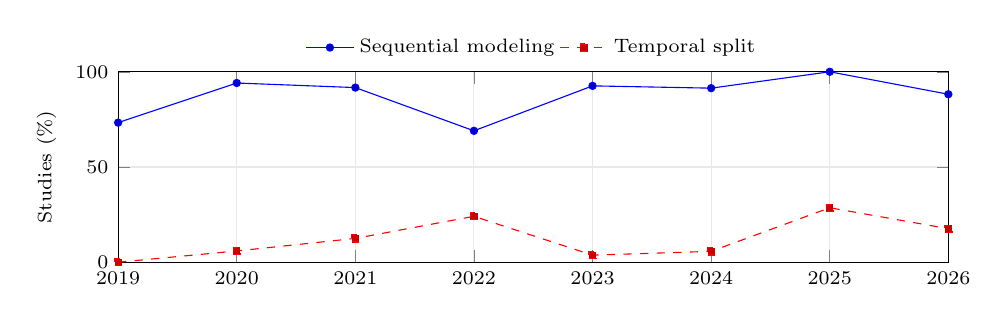
\begin{tikzpicture}
\begin{axis}[width=\columnwidth, height=4.0cm, xmin=2019, xmax=2026,
  xtick={2019,2020,2021,2022,2023,2024,2025,2026},
  xticklabel style={/pgf/number format/1000 sep=}, ytick={0,50,100}, ymin=0, ymax=100,
  tick label style={font=\scriptsize}, ylabel={\scriptsize Studies (\%)},
  legend style={font=\scriptsize, at={(0.5,1.02)}, anchor=south, legend columns=2, draw=none},
  grid=major, grid style={draw=gray!18}, mark size=1.3pt]
\addplot+[mark=*] coordinates {(2019,73.3) (2020,94.1) (2021,91.7) (2022,69.0) (2023,92.6) (2024,91.4) (2025,100.0) (2026,88.2)};
\addlegendentry{Sequential modeling}
\addplot+[mark=square*,dashed] coordinates {(2019,0.0) (2020,5.9) (2021,12.5) (2022,24.1) (2023,3.7) (2024,5.7) (2025,28.6) (2026,17.6)};
\addlegendentry{Temporal split}
\end{axis}
\end{tikzpicture}
\caption{Modeling--evaluation gap by year. Studies per year: 15, 17, 24, 29, 27, 35, 7, 17 (2019--2026). The 2025 ($n=7$) and 2026 ($n=17$) strata are small and include studies added after the original search (Appendix~\ref{sec:appendix_collection}), so their rates are not comparable to earlier years.}
\label{fig:temporal_gap}
\end{figure}

\subsection{Detailed evaluation results}
\label{sec:retained_evaluation}
These intersections refine the audit. Denominators are the relevant subsets; they are not estimates of causal effects.

\begin{table}[htbp]
\centering\small
\setlength{\tabcolsep}{2pt}
\begin{tabular*}{\columnwidth}{@{\extracolsep{\fill}}lrr@{}}
\toprule
\multicolumn{3}{@{}l@{}}{\textbf{Interpretability studies ($n=66$)}}\\
\midrule
\textbf{Evaluation} & \textbf{$n$} & \textbf{\%}\\
\midrule
Expert review          & 14 & 21.2\\
Workflow integration   & 11 & 16.7\\
Temporal split         & 5  & 7.6\\
Calibration            & 3  & 4.5\\
Prospective validation & 1  & 1.5\\
\bottomrule
\end{tabular*}
\caption{Validation within interpretability studies.}
\label{tab:interp_subset}
\end{table}

Among the 28  studies with public artifacts, 15 (53.6\%) report subject separation, eight (28.6\%) external validation, two (7.1\%) temporal splitting, none prospective validation, and 26 (92.9\%) static metrics only. Of the 19 expert-validated studies, none reports temporal, external, prospective, or calibration evaluation; all 16 that are  use static metrics only. Of the 19 temporally split studies, ten (52.6\%) report robustness, three (15.8\%) calibration, and none external validation; ten of the 16  ones (62.5\%) use static metrics only. Of the 56 studies with irregular or incomplete observations, 38 (67.9\%) report an identifiable handling strategy, 22 (39.3\%) robustness analysis, and 19 (33.9\%) both; 19 of the 38 with a handling strategy (50.0\%) never test it. These intersections separate auditability, expert usefulness, the ability to process incomplete data, and demonstrated longitudinal reliability.

\begin{figure*}[t]
\centering
\includegraphics[width=0.90\textwidth, trim=5 50 5 10, clip]{longitudinal_dataset.pdf}
\caption{Overview of longitudinal data, modalities, modeling approaches, applications, challenges, and evaluation.}
\label{fig:overview}
\vspace{-2mm}
\end{figure*}

% =====================================================================
\section{Detailed Survey Protocol}
\label{sec:appendix_methodology}

\subsection{Review Dimensions}
\label{sec:appendix_questions}
Each study is coded on 112 fields in six blocks: bibliographic metadata (source, year, access, paper type, authors, venue, DOI, URL); problem framing (task, subdomain, problem statement, objectives, temporal aspect, stated limitations, future work); data (dataset and access, size, language, modality, application area); methods (techniques, models, model type, metrics, findings, code and licence, reproducibility); longitudinal handling (missing-data strategy, temporal challenges, interpretability and translation characteristics); and evaluation (observed limitations and validation strategies). Each of the last four blocks has a primary category, a multi-label list, an \emph{evidence/rationale} field citing the supporting passage, and one binary indicator per category.

\subsection{Source Selection and Scope}
\label{sec:appendix_sources}
IEEE Xplore contributes engineering, imaging, signal-processing, and clinical-informatics research, including conference papers and journal articles. The ACL Anthology (ACL, AACL, COLING, EACL, EMNLP, LREC, NAACL, TACL, and co-located workshops including CLPsych, BioNLP, KnowFM, and SemEval) contributes language-centred research. Eligible studies are English-language full papers published from January 2019 to the search freeze of October 12, 2026; the earliest included study is from 2019. Foundational and later references supply context only and do not enter any denominator. The sample is neither source-balanced nor exhaustive (Appendix~\ref{sec:appendix_source_analysis}).

\subsection{Literature Collection and Search Strategy}
\label{sec:appendix_collection}
\paragraph{ACL Anthology.} We queried the Anthology's official XML metadata (\url{https://github.com/acl-org/acl-anthology}), from which \url{aclanthology.org} is built, rather than scraping web pages: one collection file per event provides titles, abstracts, authors, DOIs, venues, tracks, and publication months, so a full scan needs a few hundred file downloads instead of thousands of page requests. Downloaded files are cached and validated, and failed downloads are retried. The search ran in two rounds with the same retrieval rule: a paper is retrieved if its title contains \emph{longitudinal} (case-insensitive).
\begin{itemize}[leftmargin=*,nosep]
\item \textbf{Round 1 (January 2019--February 2025).} For each year, the script loaded every conference collection of ACL, AACL, COLING, EACL, EMNLP, LREC, and NAACL, handling both identifier schemes (pre-2020 letter codes such as \texttt{P19} for ACL 2019 and \texttt{D19} for EMNLP 2019; later identifiers such as \texttt{2024.acl}), all Findings volumes, and every workshop volume that the Anthology lists as co-located with a target conference.
\item \textbf{Round 2 (March 2025--October 12, 2026).} The script loaded the 2025--2026 collections of the same seven conferences and their Findings volumes (e.g., \texttt{2025.acl}, \texttt{2025.findings}; AACL Findings appear under \texttt{ijcnlp} in 2025). Co-located workshops were not scanned in this round.
\end{itemize}
In both rounds, volumes were filtered by publication month to respect the window, the front-matter entry of each volume was skipped, and each match was exported with title, authors, DOI, pages, abstract, venue, track (main, Findings, or workshop), and Anthology identifier. Abstracts were additionally tagged with regular-expression categories---datasets (e.g., \emph{longitudinal corpus}, \emph{user timelines}, \emph{repeated measures}), modelling (e.g., \emph{disease progression}, \emph{moments of change}, \emph{time-aware models}), evaluation (e.g., \emph{temporal drift}, \emph{time-based splits}, \emph{early detection}), and approaches (e.g., \emph{diachronic}, \emph{semantic change})---and given a weighted relevance score. Tags and scores only ordered records for screening; they never excluded any.

\paragraph{Studies identified outside the scripted search.} Ten included ACL Anthology studies were not retrievable by the two scripted rounds: four TACL articles (TACL is not among the searched collections) and six papers from 2025--2026 workshops (CLPsych, BioNLP, KnowFM, and SemEval), which Round~2 did not scan. Seven of the ten (the four TACL articles and three workshop papers) also lack \emph{longitudinal} in their titles.

\paragraph{Screening counts and deduplication.} The original search retrieved 815 records, of which 551 passed automated filtering, 520 manual screening, and 149 full-text review. The updated search added 60 records (40, 35, and 25 at the same stages; 17 ACL Anthology and 8 IEEE Xplore inclusions), giving 875, 591, 555, and 174. Records were matched by normalised title (lower-cased, punctuation removed) and by DOI where available; two IEEE Xplore papers that had each been coded twice were removed, leaving 172 unique studies (Table~\ref{tab:screening_counts_small}).

\begin{table}[!t]
\centering
\footnotesize
\setlength{\tabcolsep}{2pt}
\renewcommand{\arraystretch}{0.95}
\begin{tabular*}{\columnwidth}{@{\extracolsep{\fill}}lcccc@{}}
\toprule
\rowcolor{gray!18}
\textbf{Source} &
\textbf{Retrieved} &
\textbf{Automated} &
\textbf{Manual} &
\textbf{Included} \\
\midrule
ACL Anthology & 76  & 55  & 44  & 34  \\
IEEE Xplore   & 799 & 536 & 511 & 138 \\
\midrule
\textbf{Total} &
\textbf{875} &
\textbf{591} &
\textbf{555} &
\textbf{172} \\
\bottomrule
\end{tabular*}
\caption{Screening workflow by source. ``Included'' counts
unique studies after deduplication. The original search yielded
815/551/520 records (35/28/20 ACL Anthology; 780/523/500 IEEE
Xplore); the updated search added 60/40/35 (41/27/24 ACL
Anthology; 19/13/11 IEEE Xplore). Full-text review retained
174 records (149 original; 25 new); removing two duplicate
IEEE Xplore records leaves 172.}
\label{tab:screening_counts_small}
\end{table}

\subsection{Screening Criteria}
\label{sec:appendix_screening}
Automated screening keeps English-language full papers within the window. Manual screening keeps studies in which the same individuals, patients, users, or entities are observed repeatedly over time and that study progression, changing states, trajectories, or timelines. Full-text review requires enough detail on data, temporal structure, task, model, or evaluation to complete the coding sheet. Uses of \emph{longitudinal} that do not denote repeated observation over time (e.g., longitudinal acoustic waves, longitudinal relay protection, longitudinal foot arches) do not meet the criteria; the effect of the three such records in the coded set is reported in Table~\ref{tab:sensitivity}.

\subsection{Coding Procedure}
\label{sec:appendix_extraction}
One primary coder annotated all studies from the full text using a written codebook (Table~\ref{tab:operational_definitions}). A second reviewer conducted a pilot review of 12 studies to check the codebook and operational definitions before full coding; disagreements were resolved by discussion. Because the second reviewer did not independently code the full corpus, we do not report inter-annotator agreement.
Fields include bibliographic metadata; problem and objectives; task, domain, language, and modality; dataset access, scale, and temporal structure; techniques, models, and metrics; code and licensing; missingness; challenges; interpretability; deployment and workflow; limitations; and validation. The evidence/rationale fields record the supporting passage and decision basis.

\subsection{Coding Conventions and Denominators}
\label{sec:appendix_conventions}
An indicator counts as present only when its value begins with ``Yes''; ``No'', ``Not reported'', ``Unclear'', ``U'', and ``Not applicable'' count as absent. All categories are multi-label, and all-study rates use $N=172$.

\paragraph{Limitation block.} Fourteen studies added in the final round record observed limitations only when the authors acknowledge them, whereas the remaining 158 record a limitation whenever the practice is absent. Because the two conventions are not comparable, every limitation rate, the static-metrics-only rates, and the public-artifact analyses use the 158  studies. All other indicators use $N=172$.

\paragraph{Missing-data strategy.} ``No clear strategy'' is coded when no explicit strategy for missing or irregular observations is stated. Seven rows in the final round recorded an unknown strategy (``U'' or ``NA'') with ``No clear strategy'' set to No; these were recoded to Yes under this rule. Explicit strategies outside the five named categories (record filtering, label exclusion, missingness-aware training) are reported as ``Other explicit strategy''.

\paragraph{Practices versus limitations.} Positive practices and limitations are not complements: a study can report a narrow robustness experiment (21.5\% report robustness analysis) and still offer limited longitudinal robustness evidence (90.5\% of  studies).

\subsection{Operational Definitions}
\label{sec:appendix_operational_definitions}
\begin{table*}[!t]
\centering
\small
\setlength{\tabcolsep}{4pt}
\rowcolors{2}{gray!6}{white}
\renewcommand{\arraystretch}{1.02}
\begin{tabularx}{\textwidth}{p{3.2cm}X}
\toprule
\rowcolor{gray!18}
\textbf{Coded category} & \textbf{Operational definition} \\
\midrule
Temporal split & Evaluation preserves chronology, such that test observations occur after training observations or otherwise assess forward temporal generalization. \\
Subject-level split & No participant, patient, user, or other subject identity is shared across evaluation partitions. \\
Insufficient temporal-leakage discussion & The study does not clearly describe how future observations, post-outcome information, overlapping windows, or other chronology violations are prevented. \\
External cohort validation & Evaluation uses a distinct cohort, dataset, institution, or population not used for model development. \\
Prospective validation & Performance is evaluated on observations collected after model development under a prospective procedure. Revealing held-out retrospective records is not prospective validation. \\
Unclear missing-data handling & Relevant missing visits, values, modalities, or observation gaps lack a sufficiently explicit handling strategy. \\
Robustness analysis & Any explicit sensitivity, perturbation, stress-test, or subgroup/domain stability analysis beyond the primary evaluation. \\
Limited robustness analysis & Robustness is absent or does not meaningfully assess temporal horizons, missingness, modality dropout, cohort/site shift, or related longitudinal perturbations. \\
Static metrics only & Evaluation uses aggregate discrimination or generation metrics without horizon-aware, transition-sensitive, temporal-consistency, or longitudinal-stability assessment. \\
No fairness analysis & No quantitative subgroup or fairness evaluation is reported for demographic, clinical, linguistic, or other relevant groups. \\
Limited benchmark comparison & Evaluation lacks sufficiently diverse or task-relevant baselines to establish generality beyond a narrow comparison. \\
Limited interpretability analysis & Interpretability is absent or restricted to attribution or visualization without longitudinal stability, expert usefulness, or temporal consistency assessment. \\
Limited domain-shift analysis & The study does not explicitly test generalization across sites, populations, acquisition conditions, platforms, time periods, or other shifted domains. \\
No public reproducibility artifacts & No public code, preprocessing/split implementation, or equivalent artifact supporting reproduction is provided. \\
\bottomrule
\end{tabularx}
\caption{Operational definitions for principal judgment-based audit categories. Categories are multi-label and may co-occur.}
\label{tab:operational_definitions}
\end{table*}

\subsection{Taxonomy Construction and Operationalization}
\label{sec:appendix_taxonomy}
The five layers synthesize existing fields; they are not additional independent annotations. Regimes overlap. Repeated observations need not preserve order; long context need not represent elapsed time; subject and chronological separation are distinct. Multimodality becomes longitudinal when modality timing or availability changes. Implicit sequence handling remains distinct from explicit imputation. Horizon-aware assessment, alignment stability, and modality-dropout testing are recommendations unless an existing code measures them.

\begin{table*}[htbp]
\centering\small
\begin{tabularx}{\textwidth}{p{2.5cm}XXX}
\toprule
\textbf{Layer} & \textbf{Source fields} & \textbf{Synthesis rule} & \textbf{Quantitative status}\\
\midrule
Observation regime & Data type, dataset, temporal aspect, modality; interval, missing-visit, sparsity flags & How observations accumulate: scheduled visits, events, activity, or asynchronous modalities & Derived synthesis; regimes overlap\\
Temporal evidence & Temporal aspect, problem, objectives, challenge labels and rationale & Available identity, ordering, gaps, recurrence, progression, and alignment cues & Uses original flags, not a new prevalence variable\\
Temporal objective & Task, problem, objectives, temporal aspect, progression flag & Inference about trajectories, transitions, forecasts, summaries, representations, or multimodal change & Task-family synthesis; counts use original fields\\
Modeling inductive bias & Methods, models, model type, missing-data strategies, sequential flag and rationale & Mechanisms for ordering, time gaps, recurrence, subject effects, transitions, or alignment & Counts use original model/challenge flags\\
Evaluation requirement & Expected: synthesis from preceding layers. Observed: metrics, validation strategies, binary flags, and limitations & Compare implied evidence with independently coded reported evaluation & Recommendations are separate from observed prevalence\\
\bottomrule
\end{tabularx}
\caption{Coding-sheet provenance of the five taxonomy layers. No new independent annotations are introduced.}
\label{tab:taxonomy_operationalization}
\end{table*}

\subsection{Derived Cross-Dimensional Analyses}
\label{sec:appendix_derived_analyses}
Rates use paper-level intersections, e.g., $N(\mathrm{progression}\cap\mathrm{temporal})/N(\mathrm{progression})$. Joint validation counts conjunctions within a study, not products of marginal percentages. Breadth is $B_i=S_i+T_i+E_i+P_i+R_i+K_i$ (subject, temporal, external, prospective, robustness, calibration); it is unweighted and is not a quality score.

\paragraph{Claim-conditioned coverage.} Each coded claim implies a check: cross-subject variability $\rightarrow$ subject separation; sequential modeling or progression $\rightarrow$ temporal split; domain shift or deployment $\rightarrow$ external validation; deployment $\rightarrow$ prospective validation; irregular intervals, missing visits, sparse observations, fusion, or shift $\rightarrow$ robustness; uncertainty $\rightarrow$ calibration. These are analyst-defined proxies. With $\mathcal A_i$ the implied and $\mathcal E_i$ the reported checks,
\begin{align*}
C_i&=\frac{|\mathcal A_i\cap\mathcal E_i|}{|\mathcal A_i|},\quad
C_{\rm macro}=\frac{1}{N'}\sum_i C_i,\\
C_{\rm micro}&=\frac{\sum_i|\mathcal A_i\cap\mathcal E_i|}{\sum_i|\mathcal A_i|}.
\end{align*}
The unit of $C_{\rm micro}$ is a \emph{study--check pair}, not a study. Of 172 studies, 171 have at least one implied check ($N'=171$). Micro-coverage is 89/390 pairs (22.8\%), macro-coverage 18.1\%, and median $C_i$ zero. At study level, 112 of 171 (65.5\%) satisfy none of their implied checks, 53 (31.0\%) some, and 6 (3.5\%) all. Alternative mappings change these values.

\paragraph{Static-metric and subset analyses.} Static-metric analyses condition on sequential modeling, progression, or fusion within the 158  studies. Other subsets are interpretability ($n=66$), public artifacts ($n=28$ of 158), expert review ($n=19$), and temporal splitting ($n=19$). The irregular/incomplete subset ($n=56$) is the union of irregular intervals, missing visits, and sparse observations; identifiable handling means ``No clear strategy''~=~No.

\paragraph{Benchmark concentration.} Dataset aliases are matched case-insensitively in the dataset and data-type fields (ADNI variants; MIMIC-III/IV/CXR; OASIS variants; ABCD; PPMI; CLPsych; Reddit; TalkLife). Counts are 24 ADNI, 15 MIMIC, seven OASIS, seven CLPsych, seven Reddit, and four each for ABCD, PPMI, and TalkLife; their union is 60 studies (34.9\%). ADNI, MIMIC, and OASIS together cover 42 studies, compared with 130 remaining studies (Table~\ref{tab:benchmark_concentration}). Counts are multi-label.

\begin{table*}[!t]
\centering
\small
\setlength{\tabcolsep}{4pt}
\renewcommand{\arraystretch}{0.95}
\rowcolors{2}{gray!6}{white}
\begin{tabular*}{\textwidth}{@{\extracolsep{\fill}}lrrrrrrr@{}}
\toprule
\rowcolor{gray!18}
\textbf{Dataset group} & \textbf{$n$} & \textbf{Subject} & \textbf{Temporal} & \textbf{External} & \textbf{Prospective} & \textbf{Robustness} & \textbf{Calibration} \\
\midrule
ADNI/MIMIC/OASIS & 42  & 59.5 & 2.4  & 26.2 & 2.4 & 28.6 & 0.0 \\
Other studies    & 130 & 28.5 & 13.8 & 7.7  & 4.6 & 19.2 & 4.6 \\
\bottomrule
\end{tabular*}
\caption{Evaluation practices for ADNI/MIMIC/OASIS studies versus the remaining corpus (\%).}
\label{tab:benchmark_concentration}
\end{table*}

\paragraph{Temporal trends and translation.} Annual rates cover 2019--2026 (Figure~\ref{fig:temporal_gap}). The translation pathway counts studies reporting decision support, then additionally deployment, workflow integration, expert validation, and prospective validation within the same study. Independent prevalence and cumulative intersections are different quantities (Table~\ref{tab:translation_maturity}).

\begin{table}[!t]
\centering
\small
\setlength{\tabcolsep}{2.8pt}
\renewcommand{\arraystretch}{0.92}
\rowcolors{2}{gray!6}{white}
\begin{tabular}{p{2.6cm}rr|rr}
\toprule
\rowcolor{gray!18}
& \multicolumn{2}{c|}{\textbf{Individual}} & \multicolumn{2}{c}{\textbf{Cumulative}} \\
\textbf{Stage} & \textbf{$n$} & \textbf{\%} & \textbf{$n$} & \textbf{\%} \\
\midrule
Decision support        & 77 & 44.8 & 77 & 44.8 \\
Deployment              & 38 & 22.1 & 20 & 11.6 \\
Workflow integration    & 21 & 12.2 & 12 & 7.0 \\
Human expert validation & 19 & 11.0 & 5  & 2.9 \\
Prospective validation  & 7  & 4.1  & 0  & 0.0 \\
\bottomrule
\end{tabular}
\caption{Translation maturity profile: independent prevalence versus the cumulative validation pathway ($N=172$).}
\label{tab:translation_maturity}
\end{table}

\subsection{Source Imbalance, Sensitivity, and Stratified Analysis}
\label{sec:appendix_source_analysis}
The corpus has 138 IEEE Xplore (80.2\%) and 34 ACL Anthology (19.8\%) studies. ACL Anthology studies use temporal splits more often (26.5\% vs.\ 7.2\%) but none reports external or prospective validation (Table~\ref{tab:crossdim_validation}). Among  studies, public artifacts appear in 35.7\% of ACL Anthology and 13.8\% of IEEE studies. The strata are small and unbalanced, so these comparisons are descriptive, not causal, and corpus-wide percentages mainly reflect computational-health work.

\begin{table}[!t]
\centering\footnotesize
\setlength{\tabcolsep}{3pt}
\begin{tabular*}{\columnwidth}{@{\extracolsep{\fill}}lrr@{}}
\toprule
\textbf{Rate (\%)} & \textbf{All} ($n{=}172$) & \textbf{Excl.\ 3} ($n{=}169$)\\
\midrule
Sequential modeling      & 86.6 & 86.4 \\
No missing-data strategy & 59.3 & 58.6 \\
Subject separation       & 36.0 & 36.7 \\
Temporal split           & 11.0 & 11.2 \\
External validation      & 12.2 & 12.4 \\
Prospective validation   & 4.1  & 4.1 \\
Robustness               & 21.5 & 21.9 \\
Calibration              & 3.5  & 3.6 \\
Subject + temporal       & 5.8  & 5.9 \\
Coverage, $C_{\rm micro}$ & 22.8 & 23.0 \\
\bottomrule
\end{tabular*}
\caption{Sensitivity analysis excluding three records in which \emph{longitudinal} does not denote repeated observation over time (acoustic waves, relay protection, foot arches). No conclusion changes.}
\label{tab:sensitivity}
\end{table}

\subsection{Reproducibility Package}
We plan to release the ACL Anthology search scripts, the codebook, the coding sheet, and the analysis script that regenerates every number and table in this paper from the coding sheet.

% =====================================================================
\section{Supplementary Synthesis and Recommendations}
\label{sec:appendix_synthesis}

\subsection{Evaluation Recommendations}
\label{sec:appendix_evaluation_recommendations}
The audit indicates that longitudinal evaluation should assess chronology, subject independence, missingness, uncertainty, and domain generalization, not only predictive performance. Table~\ref{tab:benchmark_recommendations} summarizes the principles, which apply in proportion to the claims a study makes.

\begin{table}[!t]
\centering
\small
\setlength{\tabcolsep}{2.8pt}
\renewcommand{\arraystretch}{0.92}
\rowcolors{2}{gray!6}{white}
\begin{tabular}{p{2.0cm}p{4.8cm}}
\toprule
\rowcolor{gray!18}
\textbf{Principle} & \textbf{Recommendation} \\
\midrule
Temporal integrity & Preserve chronology and prevent future leakage~\cite{rajkomar2018scalable} \\
Subject separation & Prevent subject overlap across splits~\cite{piryani2025itshightimesurvey} \\
Robustness & Test cohorts, missingness regimes, and temporal horizons~\cite{10483639,9623284} \\
Temporal metrics & Use horizon- and transition-sensitive metrics~\cite{9338417,lazaridou2021mindgapassessingtemporal} \\
Longitudinal faithfulness & Preserve chronology and accumulated context~\cite{wu-etal-2025-unfolding,qiu-etal-2024-large} \\
Multimodal reliability & Test modality dropout and asynchronous observations~\cite{10385940,10890535} \\
Reproducibility & Report preprocessing, splits, and code availability~\cite{rajkomar2018scalable,piryani2025itshightimesurvey} \\
Generalization & Validate across populations and acquisition settings~\cite{10483639,9629798} \\
\bottomrule
\end{tabular}
\caption{Recommended evaluation principles for longitudinal modeling.}
\label{tab:benchmark_recommendations}
\end{table}

\subsection{Model-Selection Guidance}
\label{sec:appendix_model_selection}
Model choice should reflect temporal structure, sampling pattern, modalities, and evaluation objectives rather than model scale alone. Table~\ref{tab:longitudinal_taxonomy_logic} links four recurring observation regimes to the temporal evidence available, the typical objective, the required modeling bias, and the implied evaluation; Table~\ref{tab:model_selection_guide} lists model families that supply each inductive bias. Regimes are illustrative rather than mutually exclusive, and the evaluation column states recommended evidence rather than an observed prevalence.

\begin{table*}[t]
\centering
\small
\setlength{\tabcolsep}{3.2pt}
\renewcommand{\arraystretch}{1.03}
\rowcolors{2}{gray!6}{white}
\begin{tabularx}{\textwidth}{@{}>{\raggedright\arraybackslash\bfseries}p{2.35cm}>{\raggedright\arraybackslash}p{2.45cm}>{\raggedright\arraybackslash}p{2.55cm}>{\raggedright\arraybackslash}p{2.35cm}>{\raggedright\arraybackslash}p{2.75cm}>{\raggedright\arraybackslash}X@{}}
\toprule
\rowcolor{gray!18}
\textbf{Illustrative setting} & \textbf{Observation regime} & \textbf{Temporal evidence} & \textbf{Typical objective} & \textbf{Required modeling bias} & \textbf{Evaluation implication} \\
\midrule
Scheduled neuroimaging cohort & Regular clinical cohort & Repeated subject-level visits at planned intervals; progression cues & Trajectory / progression modeling & Subject effects and interpretable temporal progression & Subject-disjoint splits, calibration, uncertainty, external validation \\
Event-driven clinical records & Irregular EHR trajectory & Unequal time gaps, sparse events, and missing observations & Forecasting / risk prediction & Time-gap- and event-aware updates & Chronological splits, horizon-aware results, missingness stress tests, external validation \\
Mental-health timelines & Behavioral / language timeline & Sparse evolving histories, recurrence, and local state changes & Change detection / temporal summarization & Chronology, recurrence, and history selection & Leakage checks, chronology preservation, change-aware and long-horizon robustness \\
Longitudinal multimodal records & Asynchronous multimodal trajectory & Modalities observed at different times and frequencies; missing modalities & Multimodal progression & Cross-modal alignment and missing-modality tolerance & Modality-dropout tests, alignment stability, subject separation, external validation \\
\bottomrule
\end{tabularx}
\caption{\textit{Longitudinal taxonomy crosswalk.} Regimes may overlap; the evaluation column states recommended evidence rather than a coded prevalence.}
\label{tab:longitudinal_taxonomy_logic}
\end{table*}

\begin{table*}[!t]
\centering
\small
\setlength{\tabcolsep}{3.5pt}
\renewcommand{\arraystretch}{0.96}
\rowcolors{2}{gray!6}{white}
\begin{tabularx}{\textwidth}{@{}>{\raggedright\arraybackslash\bfseries}p{3.6cm}>{\raggedright\arraybackslash}p{5.4cm}>{\raggedright\arraybackslash}X@{}}
\toprule
\rowcolor{gray!18}
\textbf{Observation regime} & \textbf{Suitable models} & \textbf{Inductive bias supplied} \\
\midrule
Small, regular cohorts & Statistical/mixed-effects models, compact RNNs & Subject effects and interpretable temporal features \\
Irregular EHR trajectories & Time-aware RNNs, GRUs, Neural ODEs, event transformers & Time-gap and event-aware updates \\
Long behavioral/language histories & Long-context, retrieval-, or memory-augmented LLMs & Chronology, recurrence, history selection \\
Asynchronous multimodal trajectories & Fusion transformers, graph models, modality-aware encoders & Cross-modal alignment and missing-modality tolerance \\
\bottomrule
\end{tabularx}
\caption{Model families that can be adapted to supply each longitudinal inductive bias.}
\label{tab:model_selection_guide}
\end{table*}

\subsection{Extended Discussion of Longitudinal Challenges}
\label{sec:appendix_challenges}
\paragraph{Data quality, missingness, and irregular sampling.} Clinical cohorts contain missing visits and heterogeneous protocols~\cite{9342532,9377173,9374343,10635830,10069449,9983643,10635519}; EHRs contain irregular and incomplete trajectories~\cite{8904478,9006400,9679113}; and behavioral data introduce sparse activity, noisy labels, demographic uncertainty, and platform bias~\cite{harrigian-dredze-2022-now,tsakalidis-etal-2022-overview,tsakalidis-etal-2022-identifying,bayram-benhiba-2022-emotionally}. Irregular intervals affect 22.1\% of studies and sparse observations 19.8\%, yet 59.3\% state no missing-data strategy. Continuous-time and missingness-aware approaches can mitigate these effects~\cite{9871150,10340079}.
\paragraph{Population heterogeneity and multimodal alignment.} Differences across populations, sites, scanners, institutions, and linguistic environments complicate generalization~\cite{10483639,10635830,tsakalidis-etal-2022-identifying,matero-etal-2024-using}. Multimodal settings involve asynchronous imaging, physiological, clinical, and behavioral measurements~\cite{10337299,9874547,9313310,10809027,10822368,10821737}; of 22 fusion studies, 7 test robustness. Harmonization, domain adaptation, robust fusion, and subject-aware representation learning can reduce these mismatches~\cite{10385940,10890535,9711166,tseriotou-etal-2024-sig,serra-etal-2023-controllable}.
\paragraph{Scalability and temporal reasoning.} Long, irregular, high-dimensional trajectories impose substantial computational and memory demands~\cite{tsakalidis-etal-2022-identifying,hills-etal-2023-creation}. RNNs and transformers capture long dependencies but require substantial data and remain difficult to interpret~\cite{8834556,8857827,10483639}. Neural ODEs, VAEs, diffusion models, and memory-aware architectures increase temporal expressivity but often increase computational cost~\cite{9761588,10635519,10635663,9669504,8885357,9983643,8730775}.
\paragraph{Bias, fairness, and interpretability.} Cohort bias, class imbalance, and confounding can accumulate across repeated observations~\cite{10483639,10340079,9629798,9313227}, yet only 1.2\% of studies evaluate fairness. Longitudinal evaluation should assess whether errors, calibration, explanations, and trajectory predictions remain equitable across subgroups over time.
\paragraph{Privacy, consent, and governance.} Repeated clinical, imaging, genetic, and behavioral observations increase re-identification and linkage risks~\cite{8914586,9623284}. Differential privacy and synthetic data reduce exposure but may reduce utility~\cite{9474660,10821737}. Restricted access also limits reproducibility~\cite{9629798,10494110,10507968,8730775}.
\paragraph{Deployment and domain shift.} Multi-site validation appears in 1.2\% of studies, and 91.1\% of  studies provide limited domain-shift analysis. Changes in populations, scanners, coding practices, platforms, and workflows accumulate over time. Federated or privacy-preserving learning can facilitate multi-site development~\cite{9983621}, but deployment claims require explicit cross-site and cross-time testing.

\begin{figure*}[t]
\centering
\includegraphics[width=0.98\textwidth, trim=10 12 10 12, clip]{challanges.pdf}
\caption{Longitudinal data regimes, model families, challenges, and modeling implications.}
\label{fig:challenges}
\end{figure*}

\subsection{Supplementary Evaluation Figures}
\label{sec:appendix_evidence_figures}
Figures~\ref{fig:ambition_evidence}--\ref{fig:claim_eval_gap} visualize the audit in Section~\ref{sec:evaluation}. All values are computed from the paper-level coding and are descriptive.

\begin{figure*}[t]
\centering
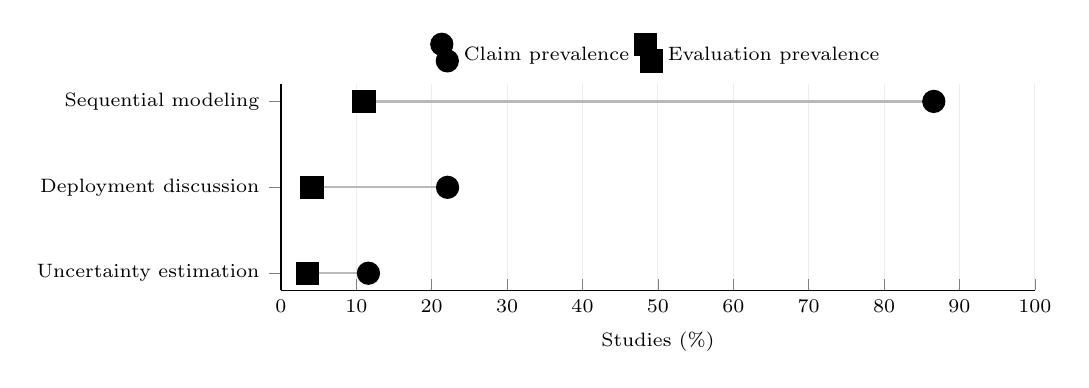
\begin{tikzpicture}
\begin{axis}[width=0.92\textwidth, height=4.2cm, xbar, xmin=0, xmax=100, xlabel={Studies (\%)},
  symbolic y coords={Uncertainty estimation, Deployment discussion, Sequential modeling}, ytick=data, y dir=normal,
  axis x line*=bottom, axis y line*=left, xmajorgrids=true, grid style={gray!15},
  tick label style={font=\scriptsize}, label style={font=\scriptsize},
  legend style={font=\scriptsize, at={(0.5,1.03)}, anchor=south, legend columns=2, draw=none}]
\draw[gray!55,thick] (axis cs:11.0,Sequential modeling) -- (axis cs:86.6,Sequential modeling);
\draw[gray!55,thick] (axis cs:4.1,Deployment discussion) -- (axis cs:22.1,Deployment discussion);
\draw[gray!55,thick] (axis cs:3.5,Uncertainty estimation) -- (axis cs:11.6,Uncertainty estimation);
\addplot[only marks, mark=*, mark size=4pt] coordinates {(86.6,Sequential modeling) (22.1,Deployment discussion) (11.6,Uncertainty estimation)};
\addlegendentry{Claim prevalence}
\addplot[only marks, mark=square*, mark size=4pt] coordinates {(11.0,Sequential modeling) (4.1,Deployment discussion) (3.5,Uncertainty estimation)};
\addlegendentry{Evaluation prevalence}
\end{axis}
\end{tikzpicture}
\caption{\textbf{Longitudinal ambition versus evaluation evidence.} Each row compares two corpus-wide marginal prevalences ($N=172$), not conditional coverage: sequential modeling (86.6\%) with temporal splitting (11.0\%), deployment discussion (22.1\%) with prospective validation (4.1\%), and uncertainty estimation (11.6\%) with calibration (3.5\%).}
\label{fig:ambition_evidence}
\end{figure*}

\begin{figure*}[t]
\centering
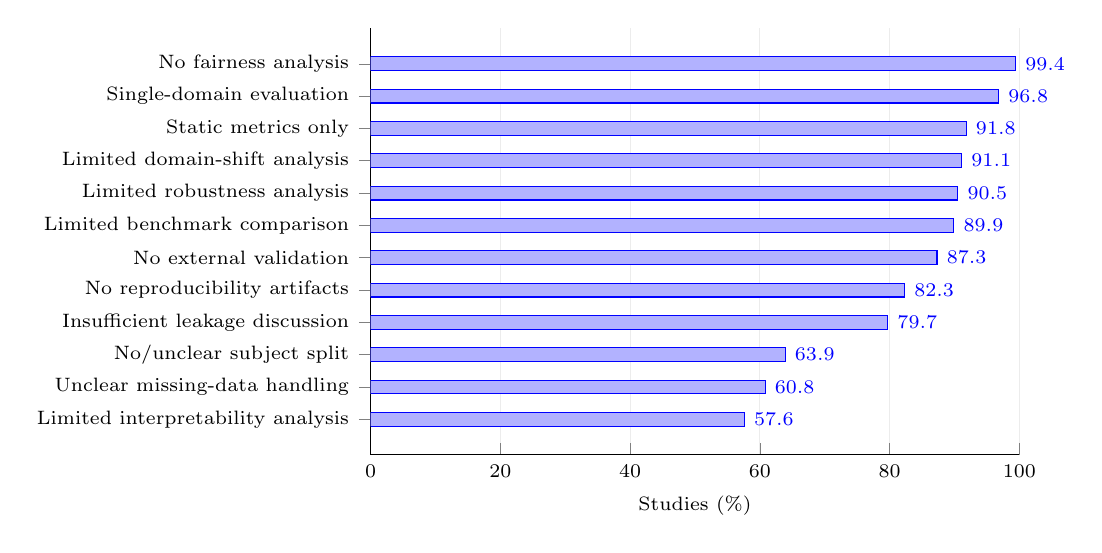
\begin{tikzpicture}
\begin{axis}[width=0.81\textwidth, height=7.0cm, xbar, xmin=0, xmax=100, xlabel={Studies (\%)},
  symbolic y coords={Limited interpretability analysis, Unclear missing-data handling, No/unclear subject split, Insufficient leakage discussion, No reproducibility artifacts, No external validation, Limited benchmark comparison, Limited robustness analysis, Limited domain-shift analysis, Static metrics only, Single-domain evaluation, No fairness analysis},
  ytick=data, y dir=normal, axis x line*=bottom, axis y line*=left, xmajorgrids=true, grid style={gray!15},
  bar width=5pt, tick label style={font=\scriptsize}, label style={font=\scriptsize}, nodes near coords, nodes near coords style={font=\scriptsize}]
\addplot coordinates {(57.6,Limited interpretability analysis) (60.8,Unclear missing-data handling) (63.9,No/unclear subject split) (79.7,Insufficient leakage discussion) (82.3,No reproducibility artifacts) (87.3,No external validation) (89.9,Limited benchmark comparison) (90.5,Limited robustness analysis) (91.1,Limited domain-shift analysis) (91.8,Static metrics only) (96.8,Single-domain evaluation) (99.4,No fairness analysis)};
\end{axis}
\end{tikzpicture}
\caption{\textbf{Where longitudinal evaluation falls short.} Prevalence of methodological and reporting limitations across the 158  studies.}
\label{fig:evaluation_blindspots}
\end{figure*}

\begin{figure}[t]
\centering
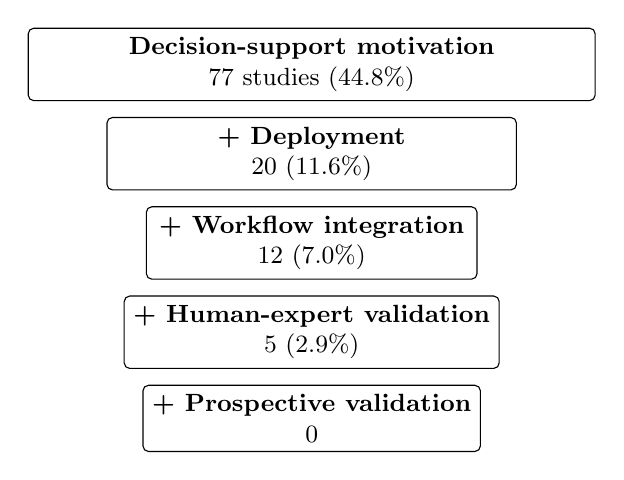
\begin{tikzpicture}[stage/.style={draw, rounded corners=2pt, minimum height=0.62cm, align=center, font=\small}]
\node[stage, minimum width=7.2cm] (a) {\textbf{Decision-support motivation}\\77 studies (44.8\%)};
\node[stage, minimum width=5.2cm, below=2mm of a] (b) {\textbf{+ Deployment}\\20 (11.6\%)};
\node[stage, minimum width=4.2cm, below=2mm of b] (c) {\textbf{+ Workflow integration}\\12 (7.0\%)};
\node[stage, minimum width=3.1cm, below=2mm of c] (d) {\textbf{+ Human-expert validation}\\5 (2.9\%)};
\node[stage, minimum width=2.2cm, below=2mm of d] (e) {\textbf{+ Prospective validation}\\0};
\end{tikzpicture}
\caption{\textbf{From clinical ambition to translational evidence.} Cumulative progression from decision-support motivation to deployment, workflow integration, human-expert validation, and prospective evaluation ($N=172$).}
\label{fig:translation_funnel}
\end{figure}

\begin{figure}[t]
\centering
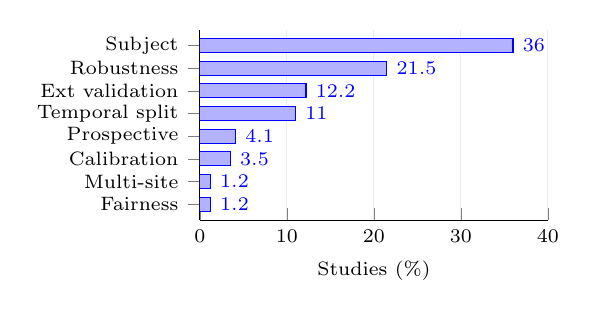
\begin{tikzpicture}
\begin{axis}[width=6.0cm, height=4.0cm, xbar, xmin=0, xmax=40, xlabel={Studies (\%)},
  symbolic y coords={Fairness, Multi-site, Calibration, Prospective, Temporal split, Ext validation, Robustness, Subject},
  ytick=data, y dir=normal, axis x line*=bottom, axis y line*=left, bar width=5pt, xmajorgrids=true, grid style={gray!15},
  tick label style={font=\scriptsize}, label style={font=\scriptsize}, nodes near coords, nodes near coords style={font=\scriptsize}]
\addplot coordinates {(1.2,Fairness) (1.2,Multi-site) (3.5,Calibration) (4.1,Prospective) (11.0,Temporal split) (12.2,Ext validation) (21.5,Robustness) (36.0,Subject)};
\end{axis}
\end{tikzpicture}
\caption{\textbf{Corpus-wide prevalence of reported validation practices} ($N=172$). Bars show independent prevalence rather than cumulative requirements; claim-conditioned coverage is in Table~\ref{tab:applicability_coverage}.}
\label{fig:evaluation_prevalence}
\end{figure}

\begin{figure}[t]
\centering
\resizebox{\columnwidth}{!}{%
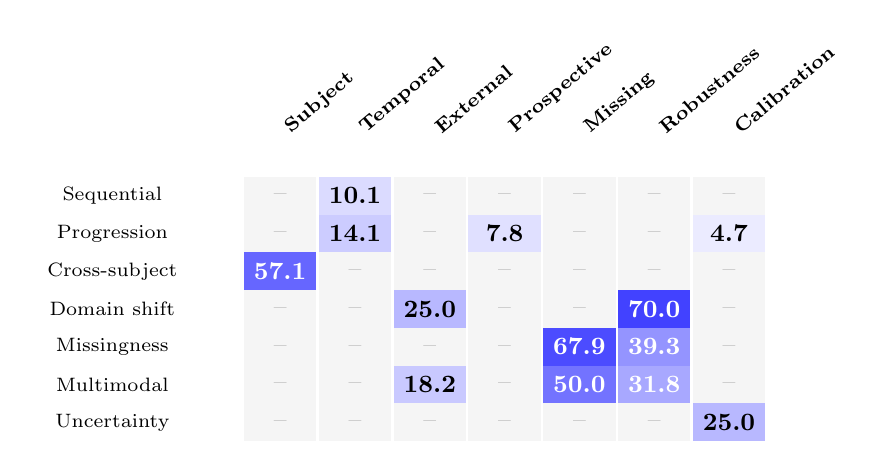
\begin{tikzpicture}[cell/.style={minimum width=0.92cm, minimum height=0.48cm, anchor=center, font=\small},
  rowlab/.style={minimum width=2.15cm, minimum height=0.48cm, anchor=east, font=\scriptsize, align=right}]
\node[font=\scriptsize\bfseries, rotate=40, anchor=west] at (0.40,0.28) {Subject};
\node[font=\scriptsize\bfseries, rotate=40, anchor=west] at (1.35,0.28) {Temporal};
\node[font=\scriptsize\bfseries, rotate=40, anchor=west] at (2.30,0.28) {External};
\node[font=\scriptsize\bfseries, rotate=40, anchor=west] at (3.25,0.28) {Prospective};
\node[font=\scriptsize\bfseries, rotate=40, anchor=west] at (4.20,0.28) {Missing};
\node[font=\scriptsize\bfseries, rotate=40, anchor=west] at (5.15,0.28) {Robustness};
\node[font=\scriptsize\bfseries, rotate=40, anchor=west] at (6.10,0.28) {Calibration};
\node[rowlab] at (-0.65,-0.48) {Sequential};
\node[rowlab] at (-0.65,-0.96) {Progression};
\node[rowlab] at (-0.65,-1.44) {Cross-subject};
\node[rowlab] at (-0.65,-1.92) {Domain shift};
\node[rowlab] at (-0.65,-2.40) {Missingness};
\node[rowlab] at (-0.65,-2.88) {Multimodal};
\node[rowlab] at (-0.65,-3.36) {Uncertainty};
\foreach \y in {-0.48,-0.96,-1.44,-1.92,-2.40,-2.88,-3.36}{
  \foreach \x in {0.40,1.35,2.30,3.25,4.20,5.15,6.10}{
    \node[cell,fill=gray!8] at (\x,\y) {\textcolor{gray!55}{--}};}}
\node[cell,fill=blue!14] at (1.35,-0.48) {\textbf{10.1}};
\node[cell,fill=blue!20] at (1.35,-0.96) {\textbf{14.1}};
\node[cell,fill=blue!12] at (3.25,-0.96) {\textbf{7.8}};
\node[cell,fill=blue!8]  at (6.10,-0.96) {\textbf{4.7}};
\node[cell,fill=blue!60,text=white] at (0.40,-1.44) {\textbf{57.1}};
\node[cell,fill=blue!28] at (2.30,-1.92) {\textbf{25.0}};
\node[cell,fill=blue!74,text=white] at (5.15,-1.92) {\textbf{70.0}};
\node[cell,fill=blue!70,text=white] at (4.20,-2.40) {\textbf{67.9}};
\node[cell,fill=blue!42,text=white] at (5.15,-2.40) {\textbf{39.3}};
\node[cell,fill=blue!55,text=white] at (4.20,-2.88) {\textbf{50.0}};
\node[cell,fill=blue!21] at (2.30,-2.88) {\textbf{18.2}};
\node[cell,fill=blue!34,text=white] at (5.15,-2.88) {\textbf{31.8}};
\node[cell,fill=blue!28] at (6.10,-3.36) {\textbf{25.0}};
\end{tikzpicture}}
\vspace{-1mm}
\caption{\textbf{Claim--evaluation alignment} ($N=172$).}
\label{fig:claim_eval_gap}
\end{figure}

% =====================================================================
\section{Supplementary Dataset Taxonomy}
\label{sec:appendix_dataset_taxonomy}
Figures~\ref{fig:dataset_examples} and~\ref{fig:taxonomy_figure} give complementary views of representative longitudinal datasets and their organization.

\begin{figure*}[!t]
\centering
\begin{minipage}[t]{0.48\textwidth}
\centering
\includegraphics[width=\linewidth]{front1.pdf}
\caption{Examples of longitudinal datasets.}
\label{fig:dataset_examples}
\end{minipage}
\hfill
\begin{minipage}[t]{0.48\textwidth}
\centering
\includegraphics[width=\linewidth]{longitudinal Paper Final Diagram (11).pdf}
\caption{Categories of longitudinal datasets.}
\label{fig:taxonomy_figure}
\end{minipage}
\end{figure*}

\subsection{Representative Dataset Catalogue}
\label{sec:appendix_dataset_catalogue}
Tables~\ref{tab:main_datasets} and~\ref{tab:main_datasets_b} summarize representative datasets across clinical cohorts, EHRs, and behavioral/social settings. Codes: M = multimodal, I = image, P = physiology, T = text; \cmark\ = public, \xmark\ = restricted. Numerical clinical variables are not natural-language text. Platform availability and controlled access require release-specific verification, and cohort enrollment is not the size of a longitudinal analysis subset.

\begin{table*}[!t]
\centering
\small\setlength{\tabcolsep}{4pt}\renewcommand{\arraystretch}{1.12}
\begin{tabularx}{\textwidth}{@{}>{\raggedright\arraybackslash}p{2.7cm}>{\raggedright\arraybackslash}p{2.6cm}>{\raggedright\arraybackslash}p{2.9cm}>{\raggedright\arraybackslash}X>{\raggedright\arraybackslash}p{2.8cm}@{}}
\toprule
\textbf{Dataset and references}&\textbf{Target; age; focus}&\textbf{Follow-up; dates; size}&\textbf{Modality code; acquisition; features}&\textbf{Origin; challenge; access}\\\midrule
\multicolumn{5}{@{}l}{\textbf{Clinical and Epidemiological Cohorts}}\\\midrule
\textbf{ADNI}\newline \cite{8857827}\newline\cite{9669504,10489807,10483639} & Alzheimer's.\newline Older.\newline Progression. & 6--12 mo.\newline 2004--present.\newline 800--1,100+. & M(I,P,T).\newline MRI, PET, CSF, genetics.\newline Imaging, biomarkers, cognition. & \includegraphics[height=.8em]{usa.png}\includegraphics[height=.8em]{canada.png}\newline Missingness, variability.\newline \cmark. \\
\textbf{OASIS}\newline \cite{10959402} & AD/aging.\newline Adult.\newline Brain atrophy. & 3--5 visits.\newline 2005--present.\newline 400--1,000+. & M(I,P,T).\newline MRI, PET, tests.\newline Imaging, cognition. & \includegraphics[height=.8em]{usa.png}\newline Small, heterogeneous.\newline \cmark. \\
\textbf{AIBL}\newline \cite{10483639} & Early AD.\newline Older.\newline Biomarkers. & 18 mo.\newline 2006--present.\newline $\sim$1,100. & M(I,P,T).\newline MRI, PET, lifestyle.\newline Imaging, lifestyle, genetics. & \includegraphics[height=.8em]{australia.png}\newline Small cohort.\newline \cmark. \\
\textbf{BLSA}\newline \cite{10635830} & Aging.\newline Older.\newline Cognitive decline. & Long-term.\newline 1958--present.\newline $\sim$1,500+. & M(I,P,T).\newline Clinical, MRI.\newline Imaging, clinical. & \includegraphics[height=.8em]{usa.png}\newline Irregular visits.\newline \cmark. \\
\textbf{PPMI}\newline \cite{10340372} & Parkinson's.\newline Adult.\newline PD progression. & Annual.\newline 2010--present.\newline $\sim$600--800. & M(I,P,T).\newline Imaging, biomarkers.\newline Multimodal. & \includegraphics[height=.8em]{global.png}\newline Imbalance.\newline \cmark. \\
\textbf{ELSA}\newline \cite{9308198} & Aging.\newline Older.\newline Socioeconomic. & Biennial.\newline 2002--present.\newline $\sim$12K. & M(P,T).\newline Surveys, clinical, biomarkers.\newline Surveys, health. & \includegraphics[height=.8em]{uk.png}\newline Limited biomarkers.\newline \cmark. \\
\textbf{ABCD}\newline \cite{10340079} & Youth.\newline Youth.\newline Development. & Annual.\newline 2016--present.\newline $\sim$11.8K. & M(I,P,T).\newline MRI, surveys.\newline Imaging, behavior. & \includegraphics[height=.8em]{usa.png}\newline Attrition.\newline \cmark. \\
\textbf{UK Biobank}\newline \cite{matthews2015uk} & Population.\newline Adult.\newline Multi-disease. & Repeat subset.\newline 2006--present.\newline 500K+. & M(I,P,T).\newline Imaging, genetics.\newline Imaging, genomics. & \includegraphics[height=.8em]{uk.png}\newline Bias.\newline \cmark. \\
\textbf{FHS}\newline \cite{tsao2015cohort} & Cardiovascular.\newline Adult.\newline Risk. & Decades.\newline 1948--present.\newline $\sim$15K. & M(P,T).\newline Exams, surveys.\newline Clinical, lifestyle. & \includegraphics[height=.8em]{usa.png}\newline Limited modalities.\newline \cmark. \\
\textbf{NACC}\newline \cite{edmonds2024data} & Alzheimer's.\newline Older.\newline Cognitive decline. & Annual.\newline 2005--present.\newline 40K+. & M(P,T).\newline Clinical, cognitive tests.\newline Clinical, cognition. & \includegraphics[height=.8em]{usa.png}\newline Missingness.\newline \cmark. \\
\bottomrule
\end{tabularx}
\caption{Representative dataset catalogue, part I: clinical and epidemiological cohorts. Sizes, dates, and access flags describe the datasets, not verified current release metadata.}\label{tab:main_datasets}
\end{table*}
\begin{table*}[!t]
\centering
\small\setlength{\tabcolsep}{4pt}\renewcommand{\arraystretch}{1.08}
\begin{tabularx}{\textwidth}{@{}>{\raggedright\arraybackslash}p{2.7cm}>{\raggedright\arraybackslash}p{2.6cm}>{\raggedright\arraybackslash}p{2.9cm}>{\raggedright\arraybackslash}X>{\raggedright\arraybackslash}p{2.8cm}@{}}
\toprule
\textbf{Dataset and references}&\textbf{Target; age; focus}&\textbf{Follow-up; dates; size}&\textbf{Modality code; acquisition; features}&\textbf{Origin; challenge; access}\\\midrule
\multicolumn{5}{@{}l}{\textbf{Electronic Health Records}}\\\midrule
\textbf{MIMIC-III}\newline \cite{8904478,beaulieu2018mapping} & ICU.\newline Adult.\newline Mortality. & ICU stay.\newline 2001--2012.\newline 60K+. & M(P,T).\newline Vitals, labs.\newline Clinical time-series. & \includegraphics[height=.8em]{usa.png}\newline Missingness.\newline \cmark. \\
\textbf{MIMIC-IV}\newline \cite{teoh2026predicting} & ICU.\newline Adult.\newline ICU modeling. & ICU stay.\newline 2008--2019.\newline 70K+. & M(P,T).\newline Vitals, labs, notes.\newline Clinical time-series. & \includegraphics[height=.8em]{usa.png}\newline Missingness.\newline \cmark. \\
\textbf{OptumLabs}\newline \cite{8904622} & Chronic.\newline Adult.\newline Population health. & Multi-year.\newline 2007--present.\newline Millions. & M(P,T).\newline Claims EHR.\newline Claims, labs. & \includegraphics[height=.8em]{usa.png}\newline Restricted.\newline \xmark. \\
\textbf{Mayo EHR}\newline \cite{9874547} & Multi-cond.\newline Adult.\newline Trajectories. & Multi-year.\newline 2000s--present.\newline Large. & M(I,P,T).\newline Imaging, notes.\newline Multimodal. & \includegraphics[height=.8em]{usa.png}\newline Restricted.\newline \xmark. \\
\textbf{eICU}\newline \cite{9926878} & ICU.\newline Adult.\newline ICU outcomes. & ICU stay.\newline 2014--2015.\newline 200K+. & M(P,T).\newline Vitals.\newline Multi-hospital. & \includegraphics[height=.8em]{usa.png}\newline Short stay.\newline \cmark. \\
\textbf{N3C}\newline \cite{9623284} & COVID.\newline All.\newline Risk. & Multi-visit.\newline 2020--present.\newline Millions. & M(P,T).\newline Labs, diagnoses.\newline Multi-site. & \includegraphics[height=.8em]{usa.png}\newline Heterogeneity.\newline \cmark. \\
\textbf{CPRD}\newline \cite{wolf2019data} & Primary care.\newline Adult.\newline Chronic disease. & Multi-year.\newline 1987--present.\newline Millions. & M(P,T).\newline GP records.\newline Longitudinal EHR. & \includegraphics[height=.8em]{uk.png}\newline Restricted.\newline \xmark. \\
\midrule
\multicolumn{5}{@{}l}{\textbf{Behavioral and Social Resources}}\\\midrule
\textbf{Reddit}\newline \cite{harrigian-dredze-2022-now} & Mental health.\newline Adult.\newline Mood tracking. & Continuous.\newline Multi-year.\newline Large. & T.\newline Posts.\newline Naturalistic text. & \includegraphics[height=.8em]{global.png}\newline Noise.\newline \cmark. \\
\textbf{TalkLife}\newline \cite{tsakalidis-etal-2022-identifying} & Peer support.\newline Youth.\newline Mood change. & Continuous.\newline Multi-year.\newline Large. & T.\newline Posts.\newline Support signals. & \includegraphics[height=.8em]{global.png}\newline Restricted.\newline \xmark. \\
\textbf{Twitter}\newline \cite{8914586} & Mood.\newline All.\newline Depression. & Continuous.\newline Multi-year.\newline Large. & T.\newline Tweets.\newline Real-world text. & \includegraphics[height=.8em]{global.png}\newline Noise.\newline \cmark. \\
\textbf{Weibo}\newline \cite{8731609} & Mood.\newline All.\newline Stress. & Continuous.\newline Multi-year.\newline Large. & T.\newline Posts.\newline Cross-cultural text. & \includegraphics[height=.8em]{china.png}\newline Platform bias.\newline \xmark. \\
\textbf{CLPsych}\newline \cite{tsakalidis-etal-2022-overview,tseriotou-etal-2025-overview,ali-etal-2026-overview} & Mental health.\newline Adult.\newline Mood shifts, self-states. & Sequential.\newline 2015--2026.\newline Small--medium. & T.\newline Timelines.\newline Annotated timelines. & \includegraphics[height=.8em]{global.png}\newline Sparse labels; DUA.\newline \xmark. \\
\textbf{EMINDS}\newline \cite{sheng2025eminds} & Behavior.\newline Adult.\newline Trajectories. & Multi-year.\newline Recent.\newline Medium. & T.\newline Posts.\newline Structured text. & \includegraphics[height=.8em]{global.png}\newline Limited validation.\newline \xmark. \\
\textbf{AnnoMI}\newline \cite{wu2022anno} & Dialogue.\newline Adult.\newline Counseling. & Sessions.\newline 2022.\newline Small. & T.\newline Dialogue.\newline Structured dialogue. & \includegraphics[height=.8em]{uk.png}\newline Small size.\newline \cmark. \\
\textbf{Open-TLS}\newline \cite{wu-etal-2025-unfolding} & Events.\newline All.\newline Timeline sum. & Temporal.\newline Recent.\newline Medium. & T.\newline Documents.\newline Multi-document. & \includegraphics[height=.8em]{global.png}\newline Complexity.\newline \cmark. \\
\textbf{LoSST-AD}\newline \cite{petti-korhonen-2024-losst} & AD speech.\newline Older.\newline Language decline. & 2--5 visits.\newline 2024.\newline Small. & T.\newline Speech.\newline Clinical speech. & \includegraphics[height=.8em]{uk.png}\newline Small cohort.\newline \xmark. \\
\bottomrule
\end{tabularx}
\caption{Representative dataset catalogue, part II: electronic health records and behavioral/social resources. Codes and caveats as in Table~\ref{tab:main_datasets}. CLPsych access is restricted under data-use agreements in the coded 2022--2026 tasks.}\label{tab:main_datasets_b}
\end{table*}

% =====================================================================
\section{Abbreviations}
\label{sec:appendix_abbreviations}
Table~\ref{tab:abbreviations_keywords} lists the abbreviations used throughout the paper.

\begin{table*}[!t]
\centering
\small
\setlength{\tabcolsep}{3pt}
\renewcommand{\arraystretch}{0.95}
\rowcolors{2}{gray!6}{white}
\begin{tabularx}{\textwidth}{@{}>{\bfseries}p{1.9cm}X!{\vrule width 0.35pt}>{\bfseries}p{1.9cm}X@{}}
\toprule
\rowcolor{gray!18}
\textbf{Abbreviation} & \textbf{Full form / description} & \textbf{Abbreviation} & \textbf{Full form / description} \\
\midrule
ADNI & Alzheimer's Disease Neuroimaging Initiative & ABCD & Adolescent Brain Cognitive Development Study \\
AD & Alzheimer's Disease & DWI & Diffusion-Weighted Imaging \\
MCI & Mild Cognitive Impairment & CBCL & Child Behavior Checklist \\
EMCI & Early Mild Cognitive Impairment & KSADS & Kiddie Schedule for Affective Disorders and Schizophrenia \\
LMCI & Late Mild Cognitive Impairment & EHR & Electronic Health Record \\
MRI & Magnetic Resonance Imaging & MIMIC-III/IV & Medical Information Mart for Intensive Care III/IV \\
PET & Positron Emission Tomography & MIMIC-CXR & MIMIC Chest X-Ray dataset \\
CSF & Cerebrospinal Fluid biomarkers & OLDW & OptumLabs Data Warehouse \\
MMSE & Mini-Mental State Examination & MCSA & Mayo Clinic Study of Aging \\
ADAS-Cog & Alzheimer's Disease Assessment Scale--Cognitive Subscale & eICU-CRD & eICU Collaborative Research Database \\
APOE & Apolipoprotein E gene & N3C & National COVID Cohort Collaborative \\
RNN & Recurrent Neural Network & SLR & Sparse Longitudinal Representations \\
LSTM & Long Short-Term Memory network & WB-SLR & Weighted Bagging of Sparse Longitudinal Representations \\
GRU & Gated Recurrent Unit & CKD & Chronic Kidney Disease \\
BiLSTM & Bidirectional Long Short-Term Memory network & ML & Machine Learning \\
OASIS & Open Access Series of Imaging Studies & DL & Deep Learning \\
AIBL & Australian Imaging, Biomarkers and Lifestyle study & NLP & Natural Language Processing \\
BLSA & Baltimore Longitudinal Study of Aging & LLM & Large Language Model \\
SVM & Support Vector Machine & PSSG-VAE & Partially Supervised Stochastic Generative Variational Autoencoder \\
GAN & Generative Adversarial Network & BIDMC & Beth Israel Deaconess Medical Center \\
CL-NMF & Cross-sectional and Longitudinal Non-Negative Matrix Factorization & OptumLabs & Mayo Clinic--UnitedHealth Group data initiative \\
PPMI & Parkinson's Progression Markers Initiative & mCCA+jICA & Multiset canonical correlation analysis with joint independent component analysis \\
rs-fMRI & Resting-State Functional Magnetic Resonance Imaging & ELSA & English Longitudinal Study of Ageing \\
DAT-SPECT & Dopamine Transporter Single-Photon Emission Computed Tomography & PD & Parkinson's Disease \\
MDS-UPDRS & Movement Disorder Society Unified Parkinson's Disease Rating Scale & SCOPA-AUT & Scales for Outcomes in Parkinson's--Autonomic \\
MoCA & Montreal Cognitive Assessment & TACL & Transactions of the Association for Computational Linguistics \\
CLPsych & Workshop on Computational Linguistics and Clinical Psychology & MoC & Moments of Change \\
\bottomrule
\end{tabularx}
\caption{Abbreviations and keywords used in the survey.}
\label{tab:abbreviations_keywords}
\end{table*}

\end{document}